\documentclass{LTHthesis}
\usepackage[T1]{fontenc}
\usepackage[utf8]{inputenc}  % Comment if you are not using utf8
\usepackage{mathptmx, helvet}
\usepackage{amssymb}
%\usepackage[swedish]{babel}  % aktivera om rapporten är på svenska
\parskip 7pt plus 2pt minus 2pt
\parindent 0pt
\usepackage[pdftex]{graphicx}
\usepackage{epstopdf}
\addbibresource{mybib.bib}  %  Comment if you don't want to use bibtex
\begin{document}
\begin{titlepages}
\author{Fredrik Karlsson \& Martin Karlsson}
\title{Advantages of Using Simultaneous Measurements of 2.4 any 5 GHz WiFi Signals for Indoor Positioning}%Temporary
\year{2014}
\month{January}
\TFRT{9999}  %%  You will get the number from the department.
\printer{Media-Tryck}  %% Probably. You may get other information from the department.
\end{titlepages}
\chapter*{Abstract}
A condensed description of my work.
\chapter*{Acknowledgements}
These people helped me a lot with my work.
\tableofcontents
\chapter{Introduction}
\section{Background}
\section{Goal}
\section{Limitations}
\section{Platform}
\section{Coordinate Systems}
\subsection{Phone Coordinate System}
\subsection{World Coordinate System}
\subsubsection{Thesis Specific Considerations}
\chapter{Background}

\chapter{Radio Signal Propagation}
%
\label{chap:RSP}
%
The performance of any wireless communication system is fundamentally limited by the properties of the radio signal. In the simplest of worlds these properties and hence the signals power, would only depend on the distance between transmitter and receiver. However, instead they vary greatly depending on the environment, from a simple line-of-sight case to a severely obstructed one, where walls, windows, furniture etc. distort the signal between transmitter and receiver. Furthermore, the signal is also affected by a large number of small-scale effects. Among them are, reflections from various surfaces, diffraction and Doppler shift due to a difference in speed between the receiver in reference to the transmitter \cite{rappaport96}. In this thesis the focus is put on obtaining good models for the indoor propagation of radio signals for the application of positioning. 

The chapter consists of a recapitulation of free space signal propagation and path loss, together with different ways of modeling these. Different sources of disturbances and their influence are discussed. 
%
\section{Free Space Propagation Model}
%
How radio signals decays with increasing transmitter-receiver (T-R) separation is of interest in many applications especially if a position is to be obtained from the received signal strength. The free space propagation model is a relatively simple model of predicting the received signal power given a certain T-R separation and a line-of-sight path in between. This model focuses on the large-scale propagation features, thus predicting the average signal strength received without small scale effects taken into account. As in most propagation models a power law function of how the signal power decays by distance is assumed$\left(\sim{1/d^2}\right)$ \cite{rappaport96}. The power received at a distance $d$ from a radiating transmitter is given by the Friis free space equation,
%
\begin{equation}
P_r(d)=\frac{P_tG_tG_r\lambda^2}{(4\pi)^2d^2L}\label{equation:friis_equation}
\end{equation}
%
where $P_r(d)$ is the received power at a T-R separation of $d$ meters, $P_t$ is the transmitted power, $G_t$ and $G_r$ is the gains of the transmitter and receiver antennas respectively, $L\geq1$ is the system loss factor which is not related to propagation i.e hardware losses and $\lambda$ is the wavelength of the transmitted signal in meters. Here the units of $P_t$ and $P_r$ are must be the same. The gains ($G_t$ and $G_r$) are dimensionless constants related to the antennas effectiveness of receiving or transmitting a signal which is related to the construction and physical properties of the antenna. The wavelength $\lambda$ is related o the frequency of the signal by,
\begin{equation}
\lambda=\frac{c}{f}=\frac{2\pi c}{\omega_c}
\end{equation} 
%
where $f$ is the signal frequency in Hertz, $\omega_c$ is the frequency in radians per second and $c$ is the speed of light in meters per second. 

The Friis equation can only be used as a predictor for $P_r$ when $d$ is in the far-field or \emph{Fraunhofer region} of the transmitting antenna \cite{rappaport96}. The far-field region of a transmitter is defined as $d>d_f$ where $d_f$ is the far-field distance defined as,
%
\begin{eqnarray}
d_f=\frac{2D^2}{\lambda} & d_f\gg D & d_f\gg \lambda \label{equation:frau_dist}
\end{eqnarray}
%
where $D$ is the largest physical dimension of the transmitting antenna.

For a radio signal with frequency ranging from 2.4 to 5 GHz (WiFi) and a largest antenna dimension $D$ of 0.1 meter, $d_f$ is in the
range of $\left[0.36,0.75\right]$  and a $d>1$ meter fulfils both the additional requirements from \ref{equation:frau_dist}.
%
\section{Path Loss}
%
The \emph{path loss}, is defined as the difference in dB between the transmitted and received power and represents the signal attenuation measured in a positive quantity of dB. If the antennas are assumed to have unity gain, an \emph{isotropic} radiator, the path loss (PL) can be obtained from \ref{equation:friis_equation} as \cite{rappaport96}, 
%
\begin{equation}
PL\left(\text{dB}\right)=10\log_{10}{\frac{P_t}{P_r}}=-10\log_{10}{\left[\frac{\lambda^2}{\left(4\pi\right)^2d^2}\right]}\label{equation:pl}.
\end{equation} 
%
It is obvious that \ref{equation:friis_equation}, and thus \ref{equation:pl} does not hold for $d=0$. To get around this large-scale fading models use a fixed distance $d_0$ with known power \cite[rappaport96]. At $d_0$ the power can either be measured or estimated from \ref{equation:friis_equation}. The distance $d_0$ needs to be in the far-field region of the transmitter, as defined in \ref{equation:frau_dist}. Furthermore, if $d_0$ is chosen to be smaller than any distance $d$ used in the application, the power at an arbitrary distance which is not $d_0$ may be related to the received power at $d_0$ by,
%
\begin{equation}
P_r(d)=P_r(d_o)\left(\frac{d_0}{d}\right)^2 \hspace{30pt} d\geq d_0\geq d_f.
\end{equation}
%
For practical reasons, as most formulas expresses powers in dB, $d_0$ is chosen to be a power of 10. In outdoor environments $d_0$ a common value is 100 meter, and in indoor environments, 1 meter is suitable. Using the latter, the power can be expressed as,
%
\begin{equation}
10\log_{10}{P_r(d)}=10\log_{10}{P_r(d_0)}-20\log_{10}{d} \hspace{30pt} d\geq d_0\geq d_f,
\end{equation}   
%
where $P_r(d_0)$ can be determined by a simple measurement at 1 meter from the transmitter. The resulting model represents the indoor line-of-sight path loss case.
%
\section{Basic Mechanisms for Signal Propagation}
%
In this section the three basic mechanisms for signal propagation, reflection, diffraction and scattering, are presented together with their respective impact on the propagation model. The presentation is rather brief recap of sections 3.5 through 3.8 in  \cite{rappaport96} and interested readers are referred there for a more in-depth description.  
%
\subsection{Reflection}
%
When a radio wave propagating through one medium encounters a medium with a different set of electrical properties, the wave is partially transmitted and partially reflected. The intensity of the transmitted and reflected wave may be related to each other through the \emph{Fresnel reflection coefficient} ($\Gamma$). This coefficient is dependent on the material properties, wave polarization, angle of incident and the frequency of the wave \cite{rappaport96}.

The requirement of a surface to be considered as a possible source of reflection is that its dimensions are much larger than the wavelength of the incident wave and typical indoor sources include walls, floor, ceiling etc. The reflections causes the signal strength to be larger in some areas of the room and less in other than the free space model predicts.
%
\subsection{Diffraction}
%
Diffraction is the property that allows waves to propagate around different obstructions, e.g round corners, travel beyond the horizon or behind obstructions. Huygens principle, which states 
\begin{quote}
 \emph{All points on a wavefront can be considered as point sources for the new wavelet.} \cite{rappaport96}
 \end{quote}
%
Where diffraction is caused by the propagation of a secondary wave into a shadowed region, and diffraction can be viewed as the wave ''bending'' around the edge of objects. Because only a fraction of the wave propagates into the shadowed region the signal strength decays rapidly when moving further into the shadowed region \cite{rappaport96}.
%
\subsection{Scattering}
%
Scattering occurs when an wave travels through an environment which consists of many objects with small dimensions compared to the wavelength per unit volume. The energy of a scattered wave is spread out in all directions from the scattering surface. Even surfaces considered flat usually posses some roughness and thus some scattering properties. 

Scattering usually contributes to a higher signal strength than the one predicted by only diffraction and reflection \cite{rappaport96}.
%
\section{Indoor Propagation Models}
%
The Friis free space equation together with the reflection, diffraction and scattering have spawned many different models for indoor signal propagation of a wide rage of complexity.
%
\subsection{Log-normal Shadowing} 
One of the more simple simple models is the log-distance path loss model
%
\begin{equation}
\log_{10}({P_r(d)})=\log_{10}({P_r(d_0)})-10n\log_{10}\left[{\frac{d}{d_0}}\right] + X_\sigma
\end{equation} 
%
where n is the path loss exponent and  $X_\sigma$ is a zero-mean Gaussian distributed random variable with standard deviation $\sigma$ (both in dB). For some typical values of $n$ for different types of environments, see table \ref{table:path_loss_n}.
%
\begin{table}
\begin{center}
\begin{tabular}{|l|c|}
\hline
\multicolumn{1}{|c|}{Signal environment} & Path loss exponent, $n$ \\
\hline
\hline
Free space & 2 \\
\hline
Indoor line-of-sight & 1.6-1.8 \\
\hline
Indoor low number of obstructions & 2-3 \\
\hline
Indoor high number of obstructions & 4-6 \\
\hline
\end{tabular}
\end{center}
\caption{Path loss exponent $n$ for different signal environments \cite{rappaport96}.}
\label{table:path_loss_n}
\end{table}
%
This models allows for some tuning for a specific environment using different values of $n$.

In figure \ref{log_norm_n_2} and \ref{log_norm_n_3_2}, measured values of the signal strength is compared to predicted ones using the log-normal shadowing model with $n=2$ and $n=3.2$ respectively, using a measured value of $\log_{10}({P_r(d_0)})= -30$. The measurements was taken while following the distance trajectory to the transmitting antenna shown in figure \ref{dist_trans}. The environment the measurement was taken i is an open office space with some obstructions.
%
\begin{figure}[!hbt]
\include{graphics}
\includegraphics[width=1\textwidth]{images/signal_model/log_norm_n_2.eps}
\caption{Measured signal strength (blue) versus signal strength modelled using the log-normal shadowing model with $n=2$ (red).}\label{log_norm_n_2}
\end{figure}
%
\begin{figure}[!hbt]
\include{graphics}
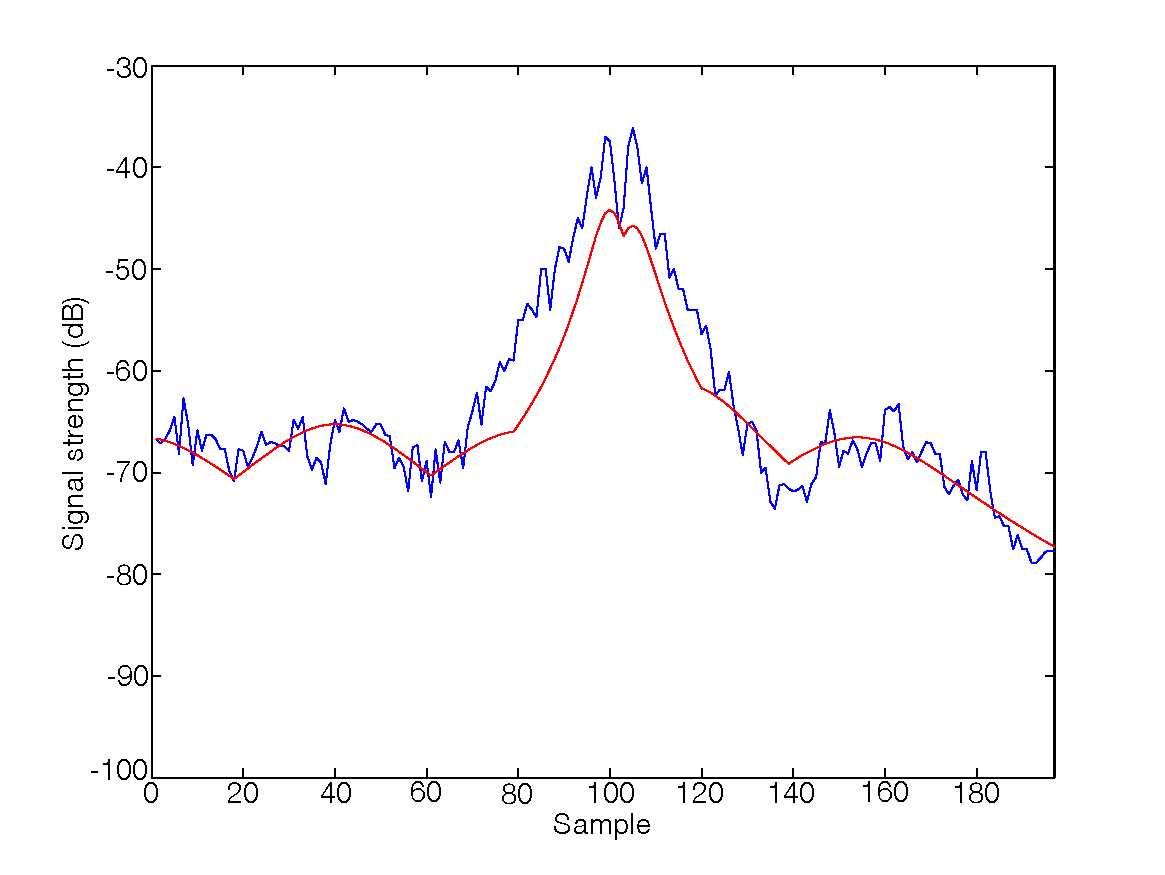
\includegraphics[width=1\textwidth ]{images/signal_model/log_norm_n_3_2}
\caption{Measured signal strength (blue) versus signal strength modelled using the log-normal shadowing model with $n=3.2$ (red).}\label{log_norm_n_3_2}
\end{figure}
%
\begin{figure}[!hbt]
\include{graphics}
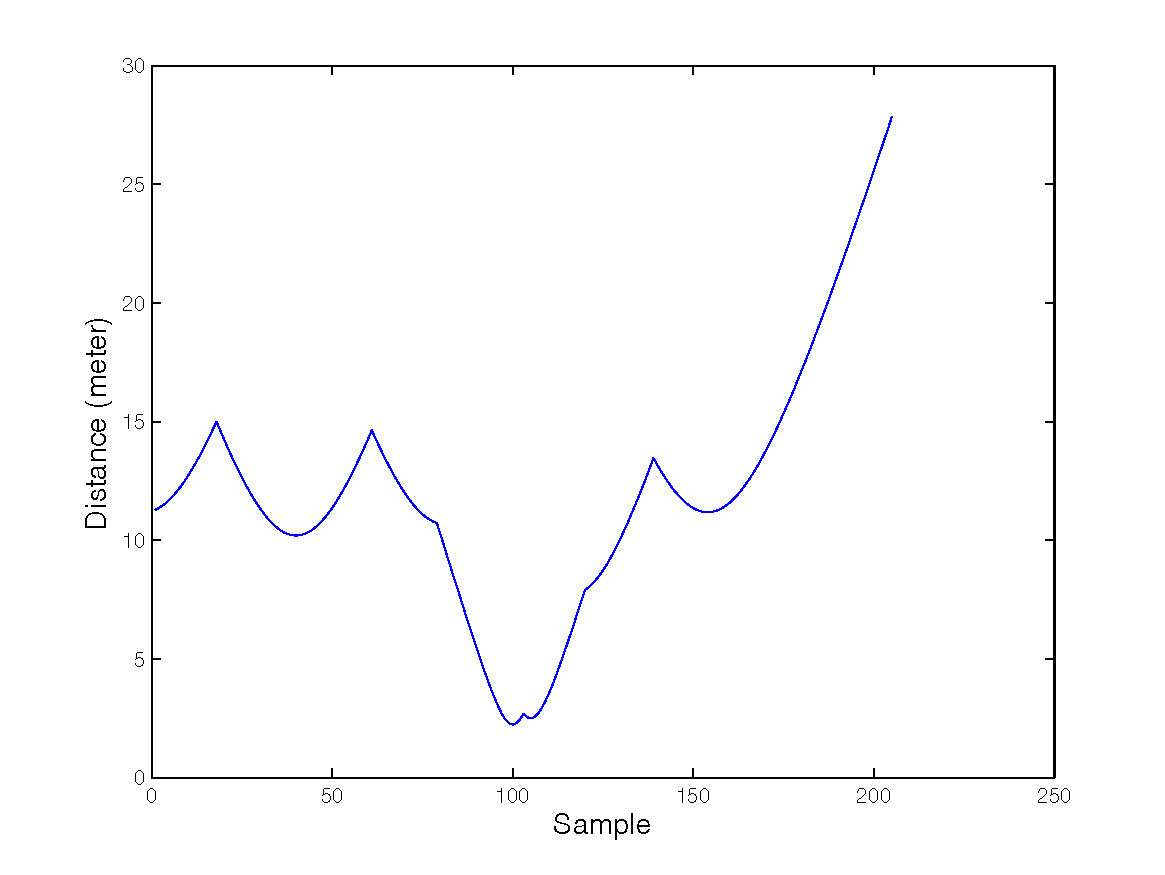
\includegraphics[width=1\textwidth ]{images/signal_model/dist_trans}
\caption{The distance to the transmitting antenna in meters used in the measurements of the signal strength}\label{dist_trans}
\end{figure}

It is obvious this model has its flaws, a low value of $n$ fails to predict good signal strength when the distance to the transmitter is fairly large and the high value does not preform satisfactory close to the transmitter. The measurement taken is similar to a real world use-case where one moves through a office space, sometimes under a transmitter in line-of-sight and sometimes being far away in an obstructed area. The flaws promotes the search for a model with better performance.
%
\subsection{Double Slope Model}
%
A simple extension of the log-normal shadowing model is combining different values of $n$ for use in various intervals of the distance to the transmitter. The most simple of these models are the double slope model where two different path loss exponent $n_1$ and $n_2$ are used together with a single break distance $d_1$ where the model changes from one to the other. This model then becomes,
\begin{subequations}
\begin{align}
\log_{10}({P_r(d)})&=&\log_{10}({P_r(d_0)})-10n_1\log_{10}\left[{\frac{d}{d_0}}\right] + X_{\sigma_1}, \hspace{5pt} d_0<d<d_1\\
\log_{10}({P_r(d)})&=&\log_{10}({P_r(d_0)})-10n_2\log_{10}\left[{\frac{d}{d_0}}\right] + X_{\sigma_2}, \hspace{5pt} d>d_1
\end{align}
\end{subequations} 
where $X_{\sigma_1}$ and $X_{\sigma_2}$ are random Gaussian distributed variables with zero mean and standard deviation $\sigma_1$ and $\sigma_2$ respectively.
 
In figure \ref{double_slope} the double slope model for $n_1=2$, $n_2=3.2$ and $d_1=10$ meter, is displayed together with measurements using the distance trajectory in figure \ref{dist_trans}.
%
\begin{figure}[!hbt]
\include{graphics}
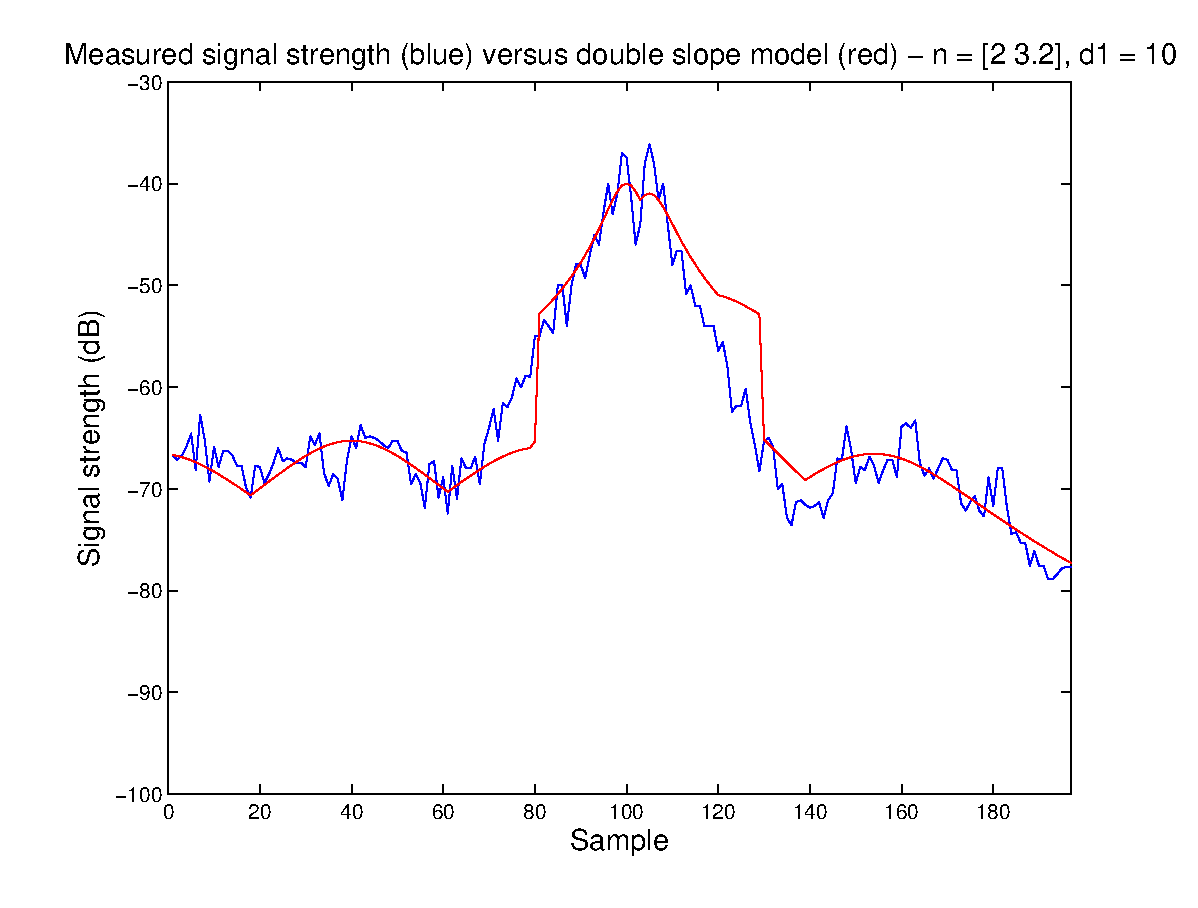
\includegraphics[width=1\textwidth ]{images/signal_model/double_slope}
\caption{Signal strength measurements (blue) versus double slope model predictions (red) with $n_1=2$, $n_2=3.2$ and $d_1=10$ meter.}\label{double_slope}
\end{figure}

This model combines the good traits from the two log-normal shadowing models, however at $d=d_1$ the model presents an undesirable ''jump'' and the prediction around $d_1$ are rather poor. Furthermore, a single $d_1$ might be hard to find for a set of transmitters and the different values of $n$ may change between the transmitters.
%
\subsection{$\alpha$-Model} %Maybe something else
%
A third attempt at modelling the signal strength is to introduce a parameter $\alpha$ multiplied with the distance $d$ in the log-normal shadowing model to account for the extra decrease in signal strength.  The model becomes,
%
\begin{equation}
\log_{10}({P_r(d)})=\log_{10}({P_r(d_0)})-10n\log_{10}\left[{\frac{d}{d_0}}\right] - \alpha d+ X_\sigma.
\end{equation}
%
where $X_\sigma$ is a zero-mean Gaussian distributed random variable with standard deviation $\sigma$.

A typical choice of $n$ for indoor conditions is 2 or slightly less, to account for the line-of-sight case when $d$ is small, see table \ref{table:path_loss_n}. The rage of $\alpha$ is around $[0.3,1.5]$ depending on the building.

This model possesses the desirable feature of only having one parameter, $\alpha$, to tune after the initial $n$ is chosen. However, it tends to underestimate the signal strength at large distances $d$, as $\alpha d$ grows linearly with $d$ while all other parts grows as the logarithm of $d$. Two simple ways to correct this easily comes to mind. Either the model can be changed to a log-normal shadowing when $d$ is large or a maximum of $\alpha d $ may be imposed. The first of these becomes     
%
\begin{subequations}
\begin{align}
\log_{10}({P_r(d)})&=\log_{10}({P_r(d_0)})-10n_1\log_{10}\left[{\frac{d}{d_0}}\right] -\alpha d+ X_{\sigma_1}, \hspace{2pt} d_0<d<d_1\\
\log_{10}({P_r(d)})&=\log_{10}({P_r(d_0)})-10n_2\log_{10}\left[{\frac{d}{d_0}}\right] + X_{\sigma_2}, \hspace{2pt} d>d_1
\end{align}
\end{subequations} 
and the second
\begin{equation}
\log_{10}({P_r(d)})=\log_{10}({P_r(d_0)})-10n\log_{10}\left[{\frac{d}{d_0}}\right] - \alpha*\min({d, d_{\text{max}})}+ X_\sigma.
\label{equation:fixed_alpha}
\end{equation}
%
Using one of these approaches, one loses some of the simplicity of having only one tunable parameter. However, these choices are simpler than for the double slope model, as there is no need to determine when the change from line-of-sight occurs. 
For \ref{equation:fixed_alpha} the predicted signals strength for $n=2$, $\alpha=0.9$ and $d_{\text{max}}=20$ is shown together with measurements in figure \ref{fixed_alpha}. 
 %
 \begin{figure}[!hbt]
\include{graphics}
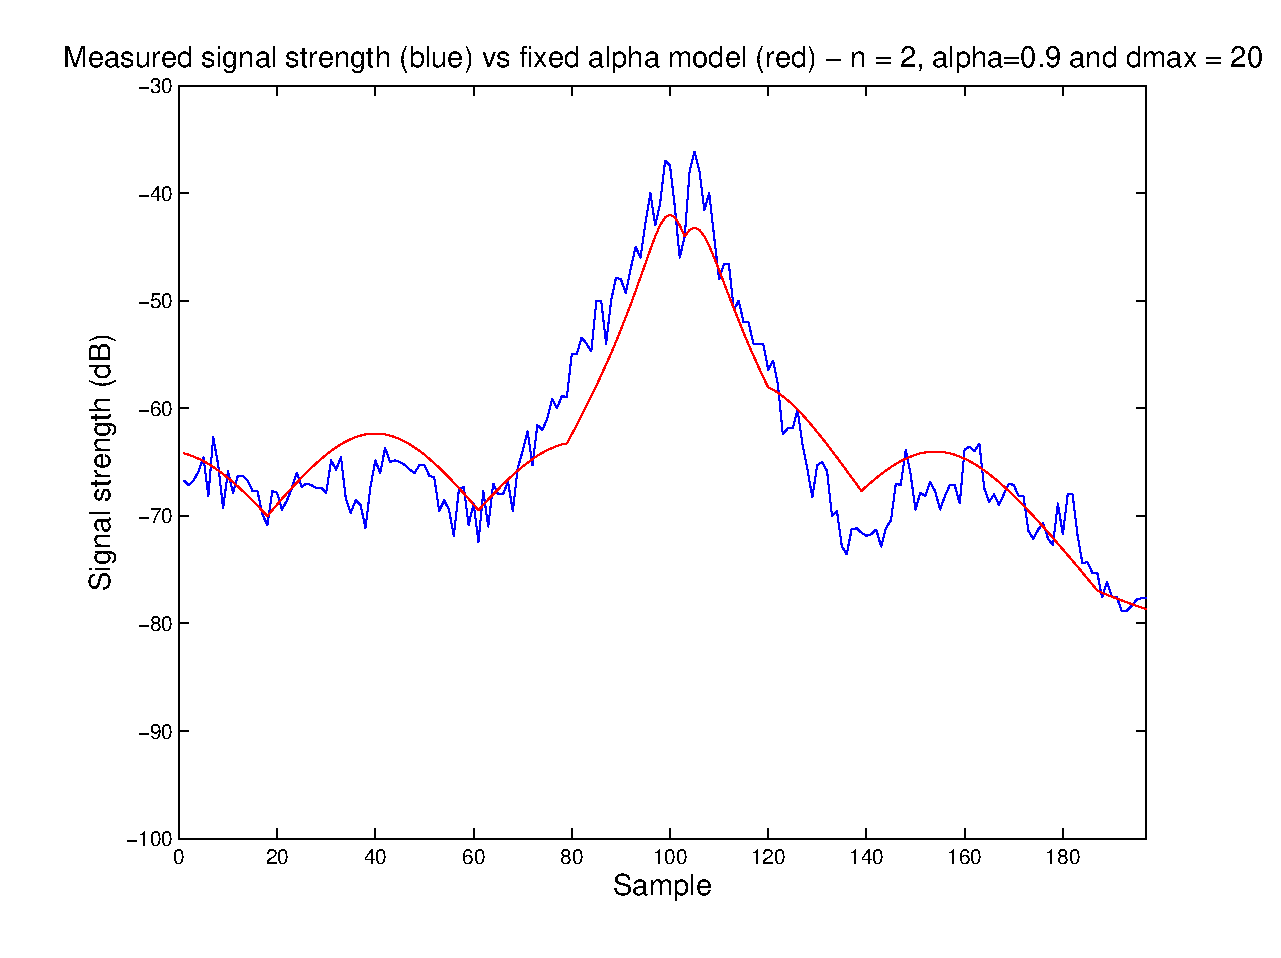
\includegraphics[width=1\textwidth ]{images/signal_model/fixed_alpha}
\caption{Signal strength measurements (blue) versus fixed $\alpha$ model predictions (red) with $n=2$, $\alpha=0.9$ and $d_{\text{max}}=20$ meter.}\label{fixed_alpha}
\end{figure}

This model predicts the signal strength satisfactory both for small and large values of $d$ while removing the ''jump'' present in the double slope model.
 %
 \section{Small Scale Fading}
 %
In addition to the large scale propagation effects described above, a radio signal usually displays a phenomena called small scale fading. The small scale fading causes the signal strength to fluctuate rapidly over small distances or short time-spans \cite{rappaport96}. This effect is caused by different waves of the transmitted signal, called \emph{multipath waves}, arriving at the receiver with a slight time difference and thus causing interference. It can be a reflected or scattered wave arriving right after the direct wave, or reflected/scattered waves from different sources reaching the receiver at different times. 

Another effect include in small scale fading is a random frequency modulation cause by different Doppler shift on different multipath signals. Sources of this is a relative movement between transmitter and receiver or movement by objects in the vicinity of the signals path. 

The description presented above is brief and for a more complete description of the small scale fading phenomena readers are referred to chapter 4 in \cite{rappaport96}.  
 %
 \section{Aspects for Positioning Applications}
 \label{sec:AfPA}
 %
 For a signal strength model to be practical for positioning, it needs to possess two properties. It needs to predict the mean signal strength at a specific distance with satisfactory precision and the variance around the mean should be sufficiently small. A few different approaches for reach this goal is available. One is to try to characterize the environment where the positioning is taking place using measurements of the signal environment i numerous points. This is feasible only when the environment are fairly uniform as the resulting model is an approximation for the entire environment. 
 
 Another approach is to, by a large set of measurements create a signal strength map of the entire environment. This is called \emph{fingerprinting} and overcomes the problem of having a changing environment, however it is impractical if used in a large area. 
 
 A third way of finding a model is to try to estimate the model parameters while the positioning is ongoing. This requires a knowledge that at some point during the positioning, the position error is known to be small, and using this knowledge finding suitable model parameters. Estimating the model has the advantaged of not being tied to a specific environment and whilst staying in the same environment the model will continue to improve. On the other hand it may not produce the best results, especially when moving between different environments or if small positioning errors are rare or hard to deem small.        
 %
\chapter{The Particle Filter}
\label{chap:PF}
%
The \emph{particle filter} or \emph{sequential Monte Carlo methods} are a set of estimation algorithms for estimating the posterior density of the state-space in a non-linear filtering problem. The particle filter uses a set of particles distributed over the state-space using a system model and state measurements are used to determine each particles probability to represent the ''true'' state of the system.  

In this chapter the non-linear filtering problem will be explained along with its solution using the particle filter. Some computational aspects will be investigated and the particle filters uses in positioning briefly discussed.
%
\section{Non-Linear Filtering Problem}
The non-linear filtering problem consists of estimating the states in a non-linear non-Gaussian model on the general form
%
\begin{subequations}
\label{equation:nonlinear_model}
\begin{align}
x_{k+1} &= f(x_k,u_k,v_k) \label{equation:nonlinear_model_first}\\
y_k&=h(x_k,u_k) + e_k
\label{equation:nonlinear_model_second}
\end{align}
\end{subequations} 
%
where $f$ and $h$ are arbitrary non-linear functions of the states $x_k$, inputs $u_k$ and process noise $v_k$, furthermore $y_k$ is the measurement at time $k$. The measurement noise $e_k$ and process noise $v_k$ are random processes with arbitrary probability density functions \cite{gson12}. 

There are a large collection of filtering methods solving this estimation problem in different ways with different restrictions. One of the most common is the \emph{Kalman filter}. This method is intuitive, simple and computationally effective, however it suffers from requiring the functions $f$ and $h$ to be linear and the probability density functions of the process $v_k$ and measurement noise $e_k$ to be zero-mean Gaussian. The \emph{extended Kalman} filter solves the problem of $f$ and $h$ being non-linear but still assumes $v_k$ and $e_k$ to be zero-mean Gaussian noise.

Here we will instead focus on another filtering approach, the \emph{particle filter} also called the \emph{Sequential Monte Carlo method}. This is a simulation based approach for solving the estimation problem \ref{equation:nonlinear_model} only requiring the probability density function of $e_k$ and $v_k$ to be known \cite{gson12,fig_fra10}.  

The particle filter consists of a set of $N$ particles $\left\{x^i\right\}_{i=1}^N$, which represents different samples of states. These particle are used to create an approximation of the distribution $p(x_k|y_{1:k})$  of the states $x_k$ given the set of measurements $y_{1:k}$. The strength of the particle filter is that the distribution $p(x_k|y_{1:k})$ can be an arbitrary one. One the other hand, to provide the same particle density the number of particle grows by the power of the number of states. I.e if you have 10 particle and one state, to provide the same density for two dimension you need 100 and for three, 1000. This makes the particle filter only suitable when the number of states is relatively small.
%
\section{The Particle Filter Process}
\label{sec:PF_process}
%
The process of the particle filter consists of three separate steps \cite{gson12}, 
\begin{enumerate}
\item \emph{Weighting of particle}: using the measurements each particle is assigned a weight corresponding to the likelihood of its states being the true ones.
\item \emph{Re-sampling}: From the existing $N$ particles create $N$ new ones by a cleaver choice.
\item \emph{State update}: Using some trajectory of the states, update the states of each particle.
\end{enumerate}
%
\begin{figure}[!hbt]
\include{graphics}
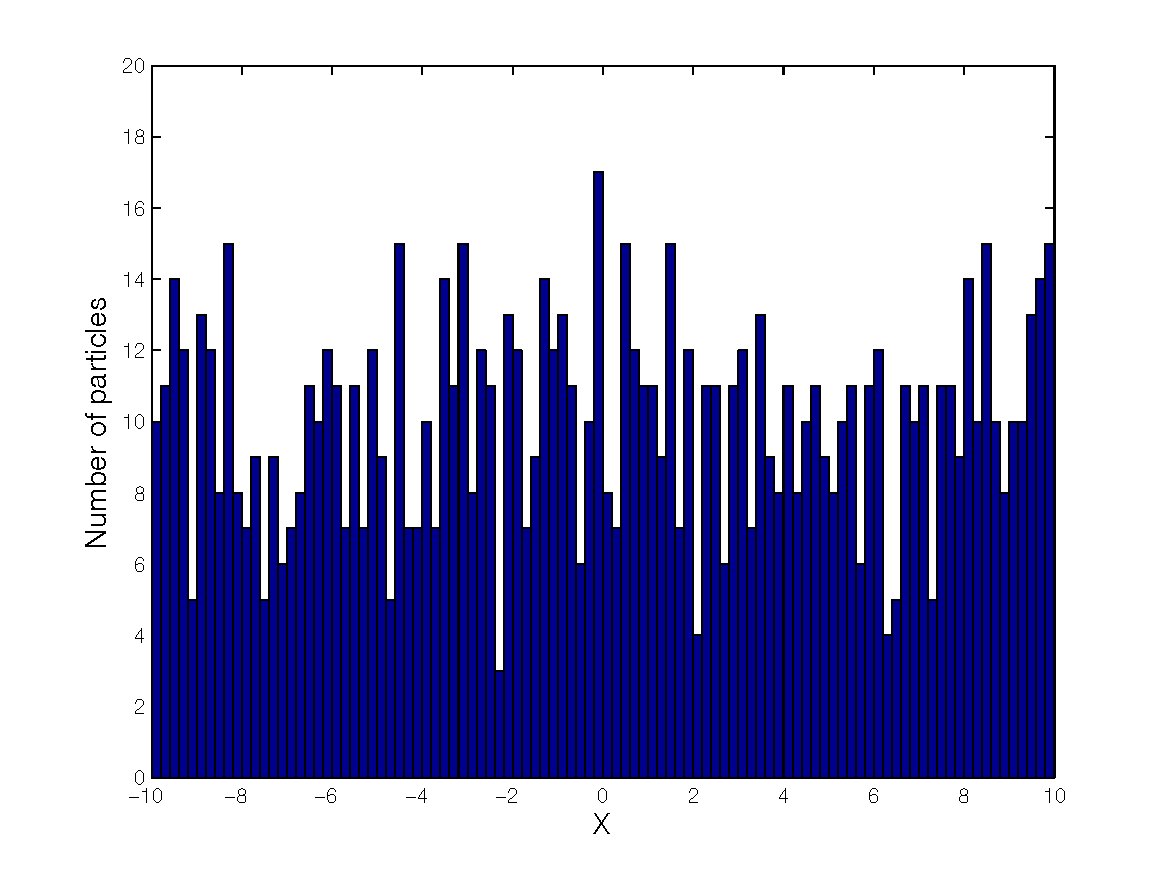
\includegraphics[width=1\textwidth ]{images/PF/hist_ini_dist}
\caption{Histogram over the initial particle distribution in range $[-10,10]$ using 100 bins}\label{hist_ini_dist}
\end{figure}
%
In the following sections these steps will be explored more in-depth along with a simple one dimensional example using $N=1000$ particles. We start by distributing the particles using an uniform distribution in the range $[-10,10]$, using $0$ as our true state and Gaussian distributed zero-mean random variable with standard deviation 1 as the measurement noise, $e_k$ from equation \ref{equation:nonlinear_model_second}. The initial particle distribution is displayed in figure  \ref{hist_ini_dist}
%
\subsection{Computing the Weights}
%
Given that the measurement noise $e_k$ is assumed to be known, the weighting of the particles is a straight forward process. For each measurement $y^l_{1:k}$ compute the probability $p^l(x^i_k|y^l_{1:k})$ that the particle $x^i$ has the true set of states. Then the total probability for each particle is,
%
\begin{equation}
p(x^i_k|y_k)=\prod_{l=1}^{L}p^l(x^i_k|y^l_{1:k}), 
\end{equation}
%
where $L$ is the number of measurements. It is also useful to have the probabilities satisfying,
%
\begin{equation}
\sum^{N}_{i=1}p(x^i_k|y_k)\equiv 1
\end{equation}
%
as to have the probabilities normalized.
%
\begin{figure}[!hbt]
\include{graphics}
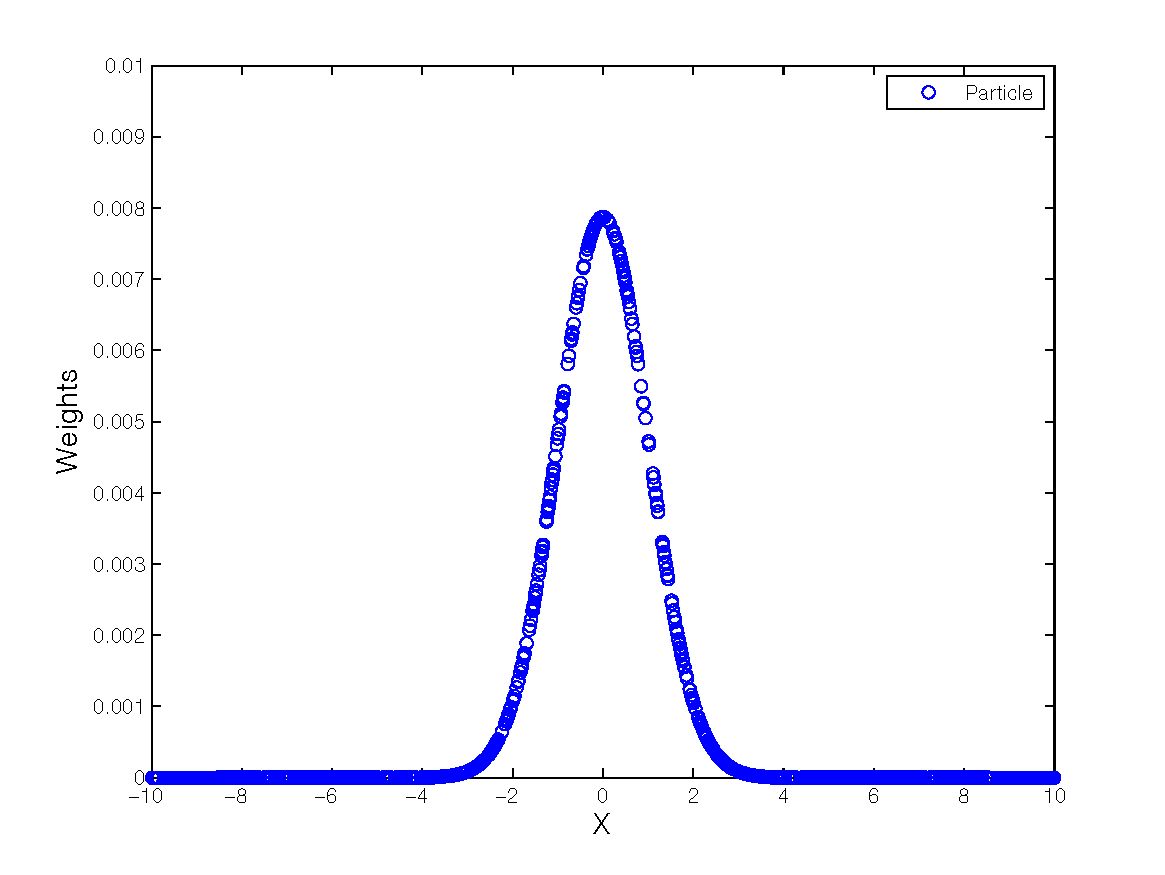
\includegraphics[width=1\textwidth ]{images/PF/particle_weights}
\caption{Particles versus their normalized weights.}\label{particle_weights}
\end{figure}

In figure \ref{particle_weights} the normalized weights assigned to each particle in our example is displayed. It comes as no surprise that the weights resembles the normally distributed measurement noise. 
%
\subsection{Re-sampling}
%
The re-sampling step is introduced to eliminate the possibility for one or a few particles to be the only probable after a few iterations of the particle filter. If the re-sampling is omitted, the computing of weight and subsequent state update could dilute the particles is the state-space until only one particle is the probable one. This could be the case even if the most probable particle does not agree with the measurement. Thus purpose of the re-sampling is to use the weights to create $N$ new particles from the $N$ old ones. This can be done in many ways, one is to allow a number of the most probable particles to spawn new particles until $N$ particles is obtained. A statistically more stringent way is to compute a uniformly distributed random number $r$ between zero and one. Then, assuming the sum of all particles probabilities are one, start adding these until the sum is greater than $r$, allowing the particles causing the change to spawn a new. Using this method particles with high probabilities have a greater chance of spawning a new while particles with small weight still may create new ones.

After the re-sampling is done it is crucial to give all particles the same weight, i.e $1/N$, as to avoid the dilution of probability.
%
\begin{figure}[!hbt]
\include{graphics}
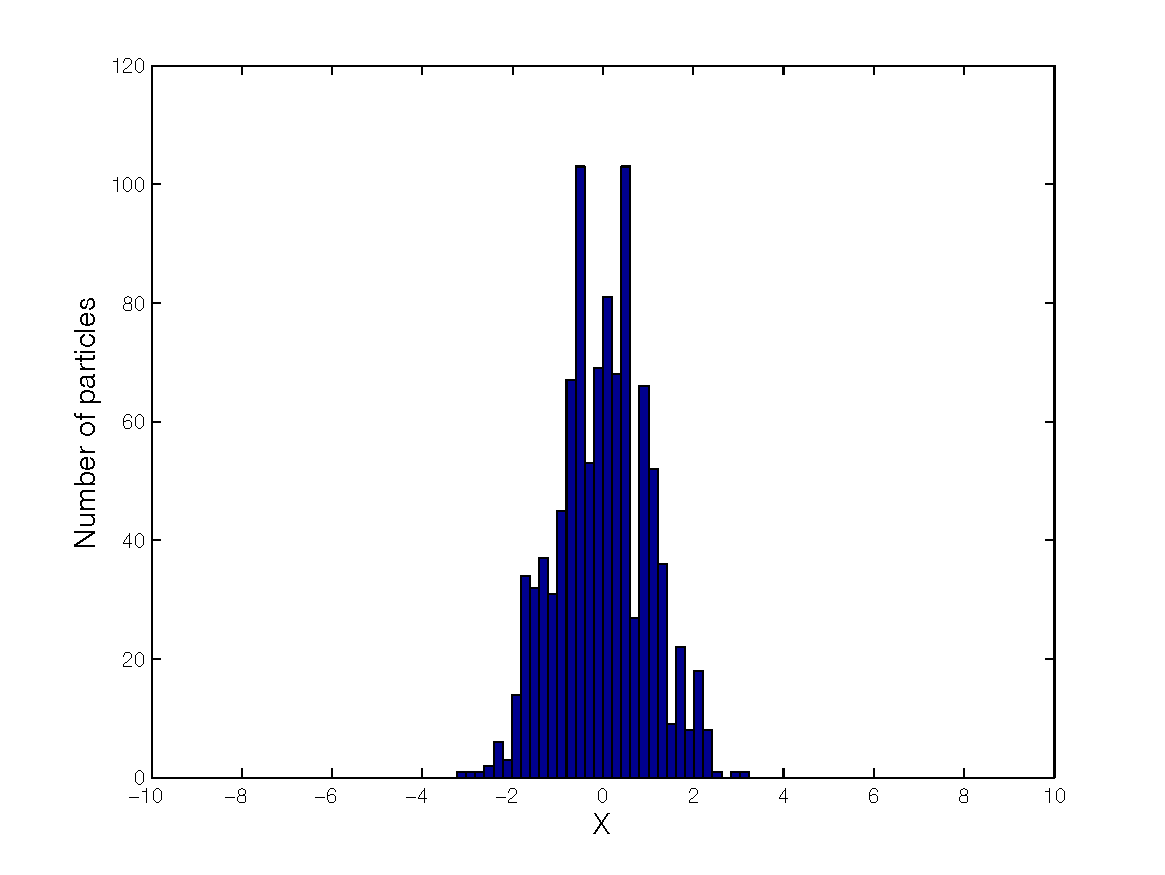
\includegraphics[width=1\textwidth ]{images/PF/hist_dist_1_itr}
\caption{Histogram over the particle distribution, after one iteration of the particle filter, in range $[-10,10]$ using 100 bins}\label{hist_dist_1_itr}
\end{figure}

After the re-sampling technique described above is applied to the particles of our example their distribution is displayed in figure \ref{hist_dist_1_itr}. After the re-sampling the states of the particles still existing tends more towards the true one, $X=0$ and the mean of the states may be used an estimation of the true one.    
% 
\subsection{State Update}
%
In the state update step some model of the system behaviour, $f(x_k,u_k,v_k)$ in equation \ref{equation:nonlinear_model_first}, is used to update the states of each particle in each time step, $k$. If the system behaviour is well known, for one or all of the states, the use  of an elaborate model improves the convergence rate of the particles and thus the estimation accuracy. This usually allows for the use of fewer particles as the approximate behaviour of the system is known and as such there is need to move particles to improbable states. 

However, if there is little or no knowledge of the states behaviour some type of random walk update can be used, only trying to capture the variance of the state over a time step. If the variance is large, this calls for a large number of particles so to keep the particle density for all probable states high. 
%
\begin{figure}[!hbt]
\include{graphics}
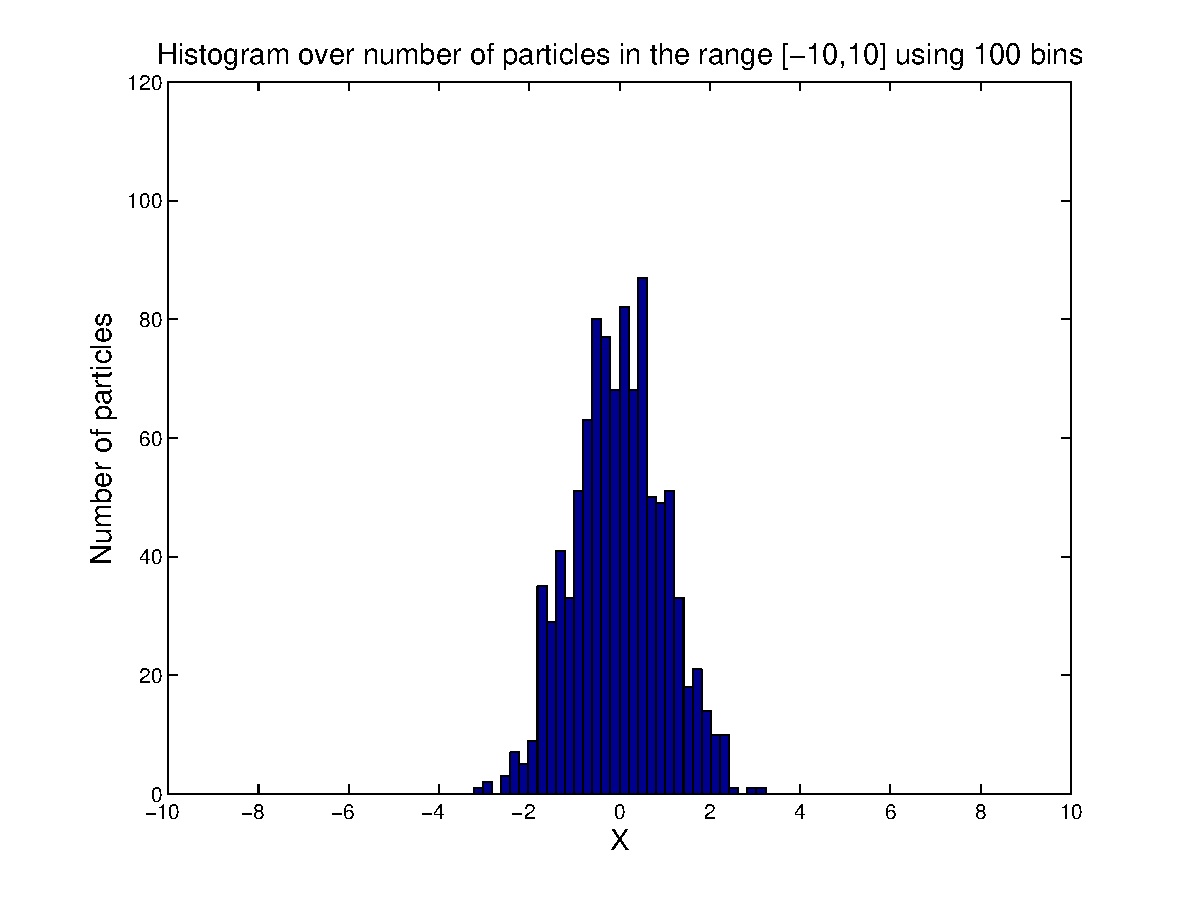
\includegraphics[width=1\textwidth ]{images/PF/hist_dist_1_itr_dyn}
\caption{Histogram over the particle distribution, after one iteration of the particle filter and a state update, in range $[-10,10]$ using 100 bins}\label{hist_dist_1_itr_dyn}
\end{figure}

In our example the ''true'' state is stationary, so the state update consists only of adding a Gaussian distributed random number with a small standard deviation ($0.1$) to each particle. This corresponds to letting each particle undergo \emph{Brownian motion}, and the resulting particle distribution may be viewed in figure \ref{hist_dist_1_itr_dyn}.
%
\begin{figure}[!hbt]
\include{graphics}
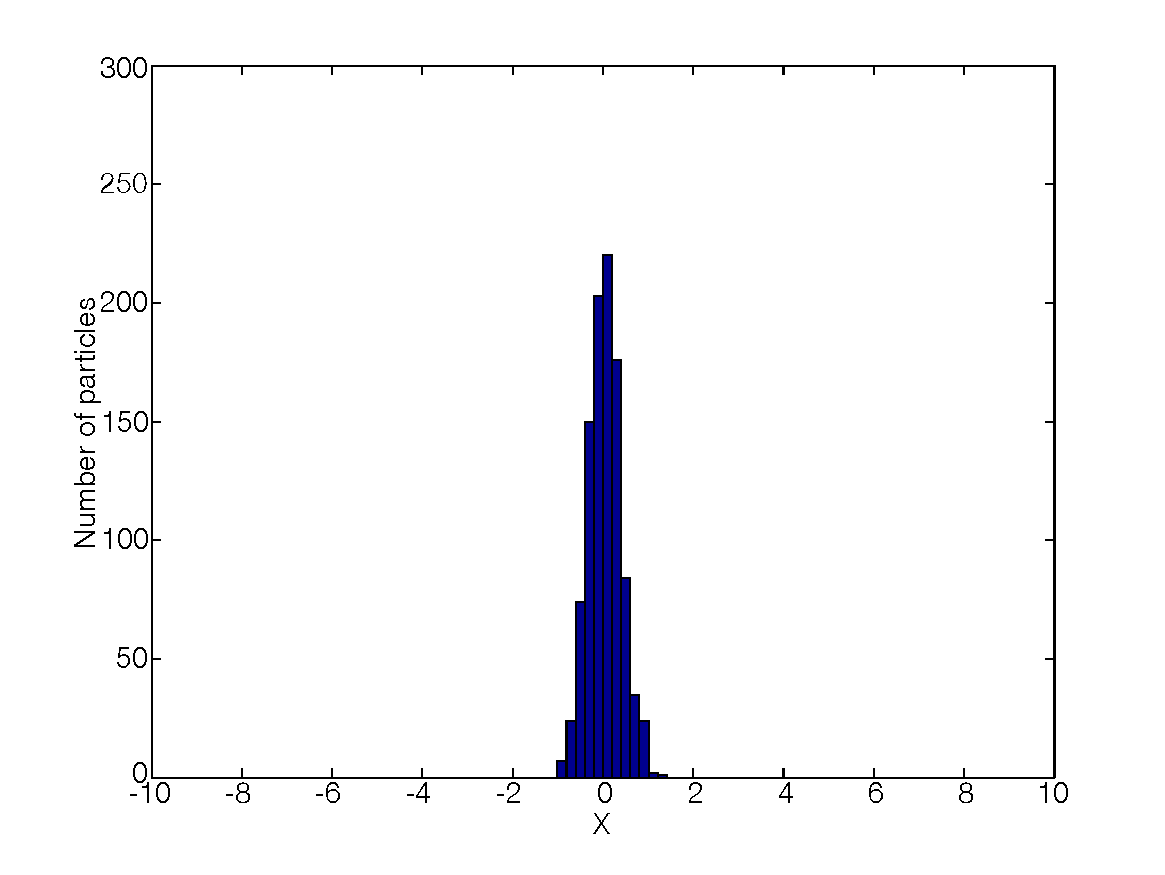
\includegraphics[width=1\textwidth ]{images/PF/hist_dist_10_itr}
\caption{Histogram over the particle distribution, after ten iteration of the particle filter, in range $[-10,10]$ using 100 bins}\label{hist_dist_10_itr}
\end{figure}

Finally, in figure \ref{hist_dist_10_itr} the particle distribution after ten iterations of the particle filter is displayed and the mean of the particle states is
\begin{equation}
\sum^{N}_{i=1}{\frac{x^i_{10}}{N}} = 0.04.
\end{equation} 
%
\section{Computational Aspects}
\label{sec:com_asp}
%
The particle filter, like most \emph{Monte Carlo} based filters, suffers from high computational complexity. Especially as the number of particles necessary to keep a fixed particle density in the state space grows as the power of the number of states. A solution to this is proposed in \cite{gson12}, where only states bearing non-linear distributions is passed throughout the particle filter and states bearing Gaussian distributions may be filtered by a different method. This is called the \emph{marginalized particle filter} and aim to keep the number of states passed to the particle filter low. 

The three steps discussed in section \ref{sec:PF_process} pose somewhat different computational difficulties. The weights needs to be calculated for each particle and thus needs to be computed $N$ times, giving a \emph{Ordo $N$} ($O(N)$) complexity. However, the calculation for each weight depends of the number of measurements $M$ giving a total complexity of $O(M*N)$. In most cases though the number of measurements is small in comparison to the number of particles and may be neglected. Another pleasant feature of the weight computation is their independence of each other, thus making parallelization of computations simple.

The re-sampling step, assuming the number of samples before and after is constant, using the algorithm described in section \ref{sec:PF_process} comprises two distinct steps. First the \emph{cumulative sum} of the weights are computed, this is of complexity $O(N)$ but can depending on the implementation be computed alongside the weights. Next, for the $N$ new particles, it is needed to determine which of the $N$ old ones is to be its clone. This is done by, for each new particle, computing a uniformly distributed random number in the range [0,1]. This random number is then compared to the cumulative sum of weights to find the index where the cumulative sum for the first time is equal to or larger than the random number. This can be done using a \emph{binary search} as the cumulative sum is sorted by its nature, giving the step complexity $O(N*\log_2{N})$. Furthermore, the particles are not entirely independent in this step, making parallelization tricky.

Updating the states is done for each particle and is dependent on the number of states $K$ along with the complexity of the state model, resulting in roughly $O(N*K)$ complexity. During this step, the particles are entirely independent, giving a possibility for parallelization.   

In all, the filter has approximately $O(N*\log_2{N})$, at least when the number of measurements $M$ and states $K$ are few compared to the number of particles.       
%
\section{Particle Filter for Positioning Application}
%
The particle filter may be successfully used in positioning applications, especially if the states and models used possesses certain features. More specific, the particle filter may be use with good results if the models are non-linear and the posterior distributions are non-Gaussian while the number of states are small \cite{gson12}. If the number of states grows the ''curse'' of dimensionality makes the use the particle filter infeasible.

 A case where the particle filter is useful is the estimation of position or position and heading in a two-dimensional space, which is the case for most indoor positioning applications. Furthermore, using signal strength from multiple sources as a measurement of position renders both a non-linear model and non-Gaussian posterior distributions further promoting the use of a particle filter. However, introducing more dynamic states e.g acceleration, unmeasured velocities or trying to filter sensor biases or drifts introduces to many dimensions. Thus, such estimations require their own filter \cite{gson12}.        
%
\chapter{Introduction to Wi-Fi} %Working title
%Citation needed
The \emph{Wi-Fi Alliance} defines WiFi as any ''wireless local area network (WLAN) products that are base on the \emph{Institute of Electrical and Electronics Engineers} (IEEE) $802.11$ standards''. However, since most WLAN products use the $802.11$ standards, in common tongue, Wi-Fi and WLAN are interchangeable.    

This chapter is intended to give an introduction to the Wi-Fi technologies and why these are of interest for indoor positioning.
%
\section{The $802.11$ Standard}
%
The (IEEE) $802.11$ standard consists of a series of techniques for over-the-air radio modulation using the same basic protocol. The standard allows different products, computers, smart-phones etc. implementing the protocol to communicate wirelessly. Historically the communication has taken place over the frequency 2.4 GHz, however in later years devices implementing 5 GHz communication protocol have become increasingly common.

The standard splits each frequency range into several channels over which the communication takes place. The frequency 2.4 GHz is split into 14 channels with 5 MHz spacing, for 5 GHz the situation is more complicated and not explained in detail. Local regulations affects which channels are allowed in a certain region.   
%
\subsection{The MAC-Address}
%
Most devices using the IEEE $802.11$ standard have an \emph{Media Access Control} (MAC) address assigned as its network address. The MAC address is usually assigned by the devices manufacturer and can be considered unique in a local area network. The address consists of twelve hexadecimal numbers and in its human readable form is presented as six groups of two hexadecimal numbers separated with either \verb|:| or \verb|-| e.g \verb|0a:1b:2c:3d:4e:5f|. They can be used to identify from which devices a signal originated.
%
\section{Wi-Fi and Positioning}
%
The Wi-Fi standard provides enticing possibilities for indoor positioning, especially in public or corporate areas. Some of the advantages over other positioning techniques is that the range of typical wireless products, like Wi-Fi access points (APs) have limited range ($\sim 30$ meter) and thus needs to be placed with relative short intervals. One of the disadvantages is that indoor signal environments often are rather complex, thus posing a harder modelling task.

Below a few different techniques for indoor positioning is presented, 
%
\begin{itemize}
\item \emph{MAC-Address}:  

Receiving a signal, and thereby a MAC-address from an AP indicates, the receiving device being  within approximately $30$. This is a rather rough positioning, but may be used to pinpoint a device to a certain area. Furthermore, receiving a signal from multiple devices should improve the positioning. 
%
\item \emph{Received Signal Strength (RSS)}:

Measuring the signal strength from a AP puts the devices not just in the vicinity, but gives a rough indication of the distance to the AP. Multiple APs may then be used to triangulated a position, but noisy measurements gives a rather large uncertainty. 
%
\item \emph{Time of Arrival (ToA)}:

If the APs and measuring device are synchronized in time, the time difference between when a message was sent and received may be used to compute the distance between device and AP. However, the the time differences involved usually are weary short ($\sim 3*10^{-9}$ seconds per meter), especially in indoor environments, requiring the time synchronization to be precise.  
%
\item \emph{Round Trip Time (RTT)}: 

A way to eliminate the requirement of synchronized APs, is to measure the time it takes for a message travel to the AP and back again, this time is called the \emph{round trip time}. As only one devices performs the time measurement the need for synchronization is eliminated, but instead the time from an AP receives a message still it sends the response needs to be known.
%
\end{itemize}
%
The techniques presented here assumes the measuring device is also performing the positioning, similar approaches are available using the APs, to position devices in the environment. Furthermore, the technologies above could be combined or used together with different technologies such as blue-tooth, NFC, rfid etc. to increase the positioning accuracy. 
In this thesis however,  the focus will be placed on the received signal strength.
%
\subsection{Received Signal Strength Indication}
%
The \emph{Received Signal Strength Indication} (RSSI) is a value indicating the short-time-average of the received signal power \cite{fig_fra10}. The RSSI is given in arbitrary units, but usually dBm, and there is no standard of how RSSI should be related to the physical properties of the received signal. 

For the RSSI to be a meaningful measurement of the received signal strength it must be related to the physical properties of the signal. Usually a measurement of the RSSI at a known distance is used together with an investigation of how the RSSI changes with the distance. The the models discussed in chapter \ref{chap:RSP} can then be applied. 
%

\subsection{RSSI Measurements in Android}

A RSSI measurement on a device running the Android operating system is initiated by an application requesting a scan of the signal environment. The operating system preforms the scan when the necessary system resources are available. Each channel specified by the IEEE $802.11$ standard and available in the current region is scanned. When a transmitter is found, a short-time average of the received signal power is measured and converted to an appropriate RSSI. The process is repeated until all reachable transmitters has been measured, and the results are returned along with information on the transmitters MAC-address, transmission frequency and a time-stamp. 

Performing a scan only when the necessary system resources are available, causes the time from a scan is request to the results are returned to be irregular. Further, an environment with many transmitters will take a longer time to scan than a environment with few.         
%
\section{Performance of 2.4 GHz Versus 5 GHz}
%
The evolution of Wi-Fi has prompted many AP to implement standards for both 2.4 and 5 GHz communications. Alongside the performance boost to devices able to use both frequencies, this poses an enticing possibility for higher performing indoor positioning. Different frequencies may, in the best case, provide two independent measurements of the distance to an AP. To investigate if this is the case, the correlation between the two frequencies must be determined.  
%
\subsection{Signal Correlation}
%
Of course, some of the signal behaviour is expected to be highly correlated. For one, the large scale distance dependent path loss is largely the same in both signals, and it is from this path loss the distance to the AP is determined. Independence is though a nice feature for the signal noise, including the \emph{small scale fading}. 

To investigate the correlation between 2.4 and 5 GHz signals, measurements could be taken, with an increasing distance, to an AP transmitting on both frequencies. After the path loss dependent behaviour is removed from the signals, the correlation of the noise could be computed.  

Such an investigation was performed, taking measurements at increasing distances, in the rang $[2,44.5]$, of the signal strength from an AP in line-of-sight. In figure \ref{noise_corr_los} the resulting noise is displayed, and computing the \emph{correlation coefficient $r_{xy}$} between the two using,
\begin{equation}
r_{xy}=\frac{\sum\limits_{i=1}^{N}{(x_i-\bar{x})(y_i-\bar{y})}}{(n-1)\sigma_x\sigma_y},
\end{equation}
where $N$ is the number of measurements, $x_i$ and $y_i$ are the 2.4 and 5 GHz measurements compensated for the path loss, $\bar x$ and $\bar y$ their means and $\sigma_x$ and $\sigma_y$ their standard deviations. The computation yields $r_{xy}=-0.31$ CONTINUED DISCUSSION ABOUT THE CORRELATION HER ? AND ANOTHER MEASUREMENT FOR NLOS? 
%
\begin{figure}[!hbt]
\include{graphics}
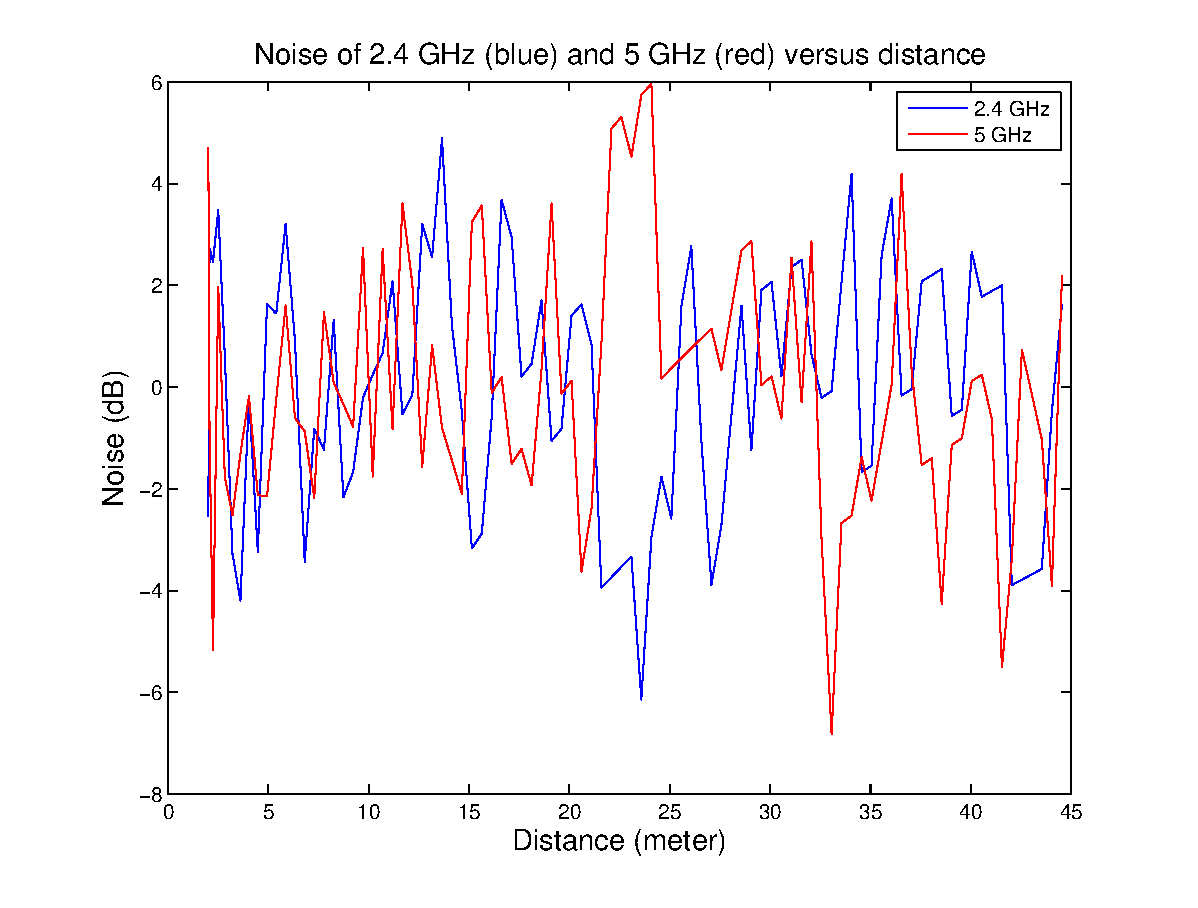
\includegraphics[width=1\textwidth ]{images/wifi/noise_corr_los}
\caption{The noise of the 2.4 and 5 GHz measurement versus distance after compensation for the path loss.}\label{noise_corr_los}
\end{figure}
%
\subsection{Difference in Modelling}
%
An extensive discussion about how path loss depends on the frequency is done in \cite{rappaport96}, the gist of which is that higher frequencies lose power faster than lower ones. The difference between 2.4 and 5 GHz is not large (a factor $\sim 2$), however some extra attention is needed to model the two. To extend the models in chapter \ref{chap:RSP} to the difference in frequency, usually different $n$ or $\alpha$, depending on choice of model, will be needed. Furthermore, an AP may transmit 5 GHz with a greater power than 2.4 GHz to mitigate some of the increased path loss, requiring measurements for both frequencies.  
%
\chapter{Indoor Positioning - Pure RSSI Approach} 
%
Using the signal propagation models described in chapter \ref{chap:RSP} in combination with the particle filter from chapter \ref{chap:PF} provides a framework for indoor positioning is obtained. This framework can then be used to perform position estimation using RSSI measurements from multiple Wi-Fi APs. 

In this chapter, the considerations about, and parameter choices for, the particle filter in the context of indoor positioning is presented. The performance is then tested in a few different environments and these tests serves as a basis for an extensive error analysis. The resulting knowledge is then used to ascertain if and how adaptive or crowd-sourced signal strength models may be used. The chapter is closed by a test of such models and their potential  advantages compared to more traditional models. 
%
\section{On Parameter Choices}
%
There are four parts of the particle filter that can be chosen by the user to some extent, the number of particle $N$, the system model, the process noise $v_k$ and the measurement noise $e_k$.
%
\subsection{System Model}
%
The process model is the most extensive choice, where both the number of states and their respective dynamics needs to be determined. Some parts of this is dependent on available measurements and how complex a model is allowed. Using only measurements of the RSSI from multiple APs, a simple model using only two states $x$ and $y$ i. e position in the plan, is used. Further, a random walk process is used to model the dynamics, resulting in the state update
%
\begin{eqnarray}
x_{k+1}&=x_k + v^x_{k+1} \\
y_{k+1}&=y_k + v^y_{k+1} 
\end{eqnarray}
%
where $v^x_k$ and $v^y_k$ is the process noise on each state. 
%
\subsection{Process Noise}
%
The process noise is, in this case, rather straight forward to choose, as it represents the spread of particles in between measurements. A normal distribution is a appropriate choice,
%
\begin{equation}
v^x_k,v^y_k\sim \mathcal{N}(\mu,\sigma^2)
\end{equation}
%
where $\mu$ represents the mean and $\sigma$ the standard deviation. In this case $\mu$ is a approximation of how far the phone travels in between measurements and $\sigma$ measures the uncertainty of this distance. A fair estimation is that a human walking travels at between 1 and 3 meters per second and given a interval $\Delta t$ between measurements $\mu = 2*\Delta t$ and $\sigma = 1*\Delta t$. Thus,
%
\begin{equation}
v^x_k,v^y_k\sim \mathcal{N}(2\Delta t, \Delta t^2)
\end{equation}
placing the new particles somewhere on an circle of radius $2\Delta t$ from the old one and spreading them out by a standard deviation of $\Delta t$.    
%
\subsection{Measurement Noise}
%
On a first glance, the measurement noise would be a fairly simple choice, i e. take a couple of sets of measurements at different distances from a AP and investigate the noise behaviour. Then use this as the measurement noise. 

FIGURES HERE!!

However, doing this gives inconclusive results, the noise seams to be dependent, both on distance from the AP and whether the AP is in line-of-sight or not. Furthermore, sometimes reflections of the signal may reach the phone in obscure ways resulting in odd measurements.

A better way is to use a zero-mean Gaussian distribution with distance dependent standard deviation, 
%
\begin{equation}
e^i_k\sim \mathcal{N}(0,\sigma(d)^2)
\end{equation}
%
where $e^i_k$ denotes the measurement noise from the $i$:th AP and $\sigma(d)^2$ is a distance dependent function. As we only pas below AP and thus never comes closer than around two meters , the noise never is deterministic and equal to zero. The function $\sigma(d)$ is to be chosen to approximate the noise found in the measurements. The lowest  standard deviation of the noise is found when the signal strength is high and is around 3 dB, and the highest standard deviation is found for $d>17$ meters and is in the worst case 20 dB. The function $\sigma(d)$ is then,
%
\begin{equation}
\sigma(d) = \left \{ \begin{array}{cc}3 + d, & 0<d<17\\ 20,  & d\geq 17\end{array}\right.
\end{equation}
%
This allows the noise to be low when the distance is short and large when the distance is large and the probability for obstructions are fairly large.
%
\subsection{Number of Particles}
%
The number of particles $N$ is the most straight forward choice, a higher $N$ directly improves the filter but increases the computational burden. If the system model is poor or the process noise is large a larger number of particles is needed to provide a sufficient particle density over the possible states.  
%
\chapter{Modelling the Kinematics} %Working title
%
Modelling the kinematics may greatly improve the performance of a positioning system, especially if the estimated position is noisy or biased. The kinematics may also be used to estimate the position in between the updates from the main positioning algorithm. The range of models stretches from simple random walk processes to estimating accelerations, velocities and position in three dimensional space using sensor fusion.

After a short description of different random walk processes, quaternions are introduced and their use in three-dimensional pose  estimation, without risk of singularities, explained. A section about positioning using only sensors, named \emph{dead reckoning}, is present after which, the chapter closes by an discussion of kinematics models used in indoor positioning and their effect on the performance.   
%
\section{Random Walk}
%
The simplest way of modelling the kinematics, aside from the trivial case of choosing not to model it at all, is to use a \emph{random walk} model for each state. In a random walk the states, $x$, undergoes time updates according to
%
\begin{equation}
x_{k+1} = x_k + v_k
\end{equation}      
%
where $v_k$ is a random process. Usually $v_k$ is considered independent for each state, and depending on the distribution and standard deviation $\sigma$, different random walk processes are obtained. How $v_k$ should be distributed is determined by the intrinsic behaviour of the states, a common choice is a normal distribution with an appropriate $\sigma$. Such a random walk is called a \emph{Gaussian random walk}, and if $\sigma$ is very small it resembles a \emph{Brownian motion}. A Gaussian random walk for three states in two dimensions, each starting in $(0\hspace{5pt}0)$, is displayed in figure \ref{rand_walk}. 
%
\begin{figure}[!hbt]
\include{graphics}
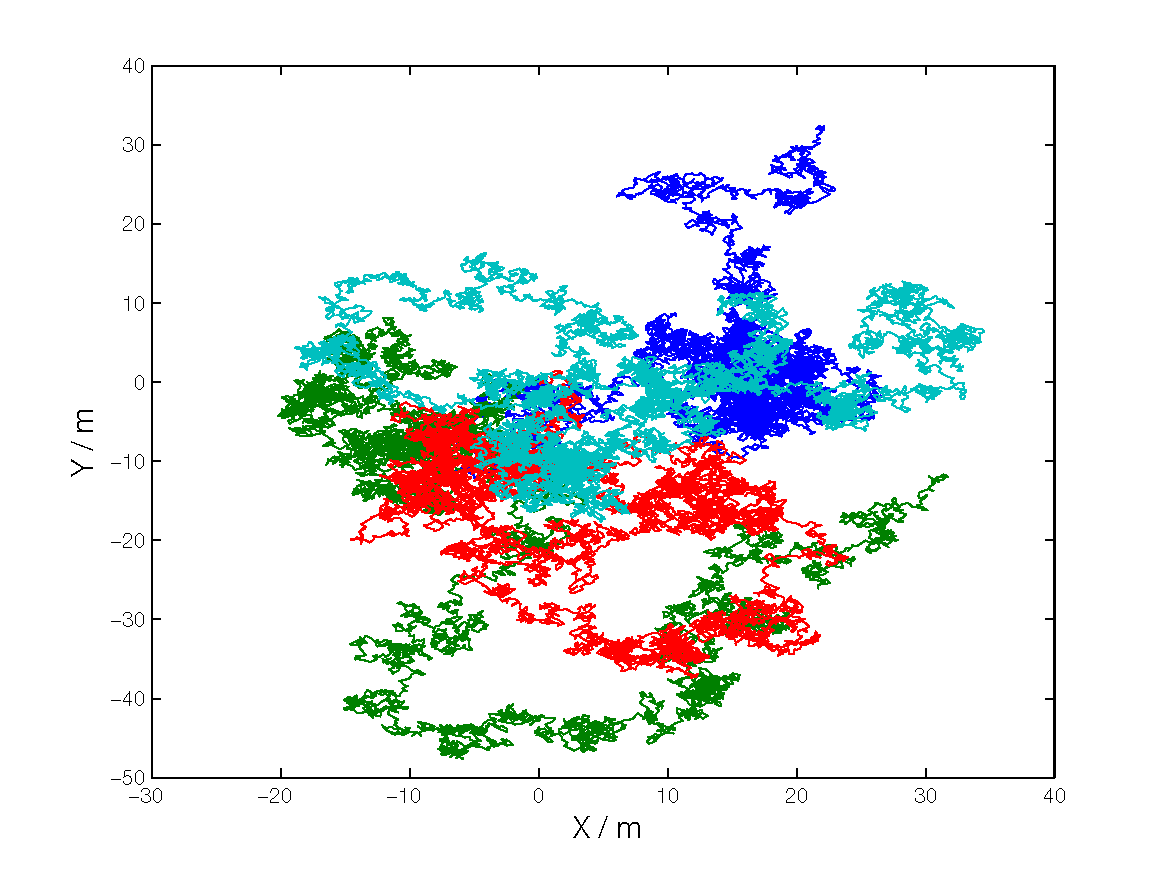
\includegraphics[width=1\textwidth ]{images/kinematic/rand_walk}
\caption{Random walk of four states using $\sigma = 1$ and $10000$ steps.}\label{rand_walk}
\end{figure}
%
\section{Quaternions}
%
The \emph{quaternions} are a extension of the complex numbers first described in 1843 by the Irish mathematician William Rowan Hamilton. They where first used in three-dimensional mechanics and today there are, among other applications, used to estimate the pose (position and direction in relation to a fixed frame) in three dimensions \cite{mann13}.
%
\subsection{Quaternion Theory}
%
As stated before quaternions are a set of numbers $q$, extending the complex number, defined as
%
\begin{equation}
q = a+bi+cj+dk, \hspace{5pt}[a,b,c,d]\in \mathbb R
\end{equation} 
%
where \emph{i, j} and $k$ are new basis elements.

Further, the basis elements obey
%
\begin{equation}
\label{equation:basis}
i^2=j^2=k^2=ijk=-1
\end{equation}
%
thus, from \ref{equation:basis} all possible of the basis multiplications can be formed according to table \ref{table:basis}.
%
\begin{table}[!hbt]
\begin{center}
\begin{tabular}{|c|c|c|c|c|}
\hline
$\times$ & $1$ & $i$ & $j$ & $k$ \\
\hline
$1$ & $1$ & $i$ & $j$ & $k$ \\
\hline 
$i$ & $i$ & $-1$ & $k$ & $-j$\\
\hline
$j$ & $j$ & $-k$ & $-1$ & $i$ \\
\hline
$k$ & $k$ & $j$ & $-i$ & $-1$ \\
\hline
\end{tabular}
\end{center}
\caption{All possible basis multiplications for quaternions.}
\label{table:basis}
\end{table}
%
A quaternion is usually seen as a four-dimensional vector consisting of a scalar $q_0$ and a vector $\vec{q} = (q_1 \; \; q_2 \; \; q_3)^T$, leading to the following notation
%
\begin{equation}
q = \left(\begin{array}{c}q_0\\ \vec{q}\end{array}\right) = \left(\begin{array}{c}q_0\\ q_1 \\ q_2 \\ q_3\end{array}\right). 
\end{equation}  
%
Quaternion multiplication is denoted by $\otimes$ and defined 
%
\begin{equation}
q\otimes r = \left(\begin{array}{c}q_0\\ \vec{q}\end{array}\right) \otimes \left(\begin{array}{c}r_0\\ \vec{r}\end{array}\right) =
\left(\begin{array}{c}q_0r_0-\vec{q} \cdot \vec{r}\\ q_0\vec{r}+r_0\vec{q}+\vec{q}\times \vec{r}\end{array}\right)
\end{equation}
%
for two quaternions $q$ and $r$, where $\cdot$ denote the scalar product and $\times$ denote the vector product. The quaternion multiplication is non-associative, meaning
%
\begin{equation}
\vec{q}\otimes \vec{r} \neq \vec{r} \otimes \vec{q}
\end{equation}
%
in general. It is, however associative
%
\begin{equation}
(\vec{q}\otimes\vec{r})\otimes\vec{s} = \vec{q}\otimes(\vec{r}\otimes\vec{s}).
\label{equation:quat_asso}
\end{equation} 
%
Further, the \emph{unit} quaternion is defined
%
\begin{equation}
{q_{\mathbf{I}}}=\left(\begin{array}{c}1\\ 0 \\ 0 \\ 0\end{array}\right)
\end{equation}
%
and the quaternion inverse $q^{-1}$ are
%
\begin{eqnarray}
q^{-1}\otimes q = q\otimes q^{-1} = q_{\mathbf{I}} &\Leftrightarrow& q^{-1} = \left(\begin{array}{c}q_0\\ -\vec{q}\end{array}\right)
\end{eqnarray}
%
Another use full definition is the quaternion norm $|q|$,
%
\begin{equation}
|q| = \sqrt{q_0^2+q_1^2+q_2^2+q_3^2 }.
\end{equation} 
%
\subsection{Quaternions Interpreted as Rotations}
%
Why a certain subset of quaternions, $|q|=1$ may be interpreted as rotations is beyond the scope of this thesis, instead here a recapitulation of how they can be use will be presented. If a reader is interested in the mechanisms involved are referred to \cite{kuip98} for an in-depth discussion of the background and theory of quaternions. 

Rotations are defined by two elements, the amount (angle) of rotation and around what axis the rotation is performed. Suppose a rotation of $\theta$ is performed around the three-dimensional unit vector $\vec n$, the quaternion representation of this would be
\begin{equation}
q = \left(\begin{array}{c}\cos{\frac{\theta}{2}}\vspace{5pt}\\ \vec{n}\sin{\frac{\theta}{2}}\end{array}\right).
\end{equation}  
%
Finding the vector $\vec v$ rotated clockwise by $\theta$ around $\vec n$, noted $\vec v_r$, by use of quaternions is done as
%
\begin{equation}
\left(\begin{array}{c}0\\ \vec{v_r}\end{array}\right) = q\otimes \left(\begin{array}{c}0\\ \vec{v}\end{array}\right) \otimes q^{-1}.
\end{equation}
%
from here on, the naming convention
%
\begin{equation}
\vec v\equiv \left(\begin{array}{c}0\\ \vec{v}\end{array}\right).
\end{equation}
%
The rotation of a vector, $\vec v$, by a quaternion, $q$ and subsequently by $p$ is equivalent to rotating $\vec v$, by the corresponding quaternion product $(p\otimes q)$. This is easily proven by multiple applications of \ref{equation:quat_asso},
%
\begin{equation}
(p\otimes q)\otimes \vec v \otimes (p\otimes q)^{-1}=p\otimes(q\otimes\vec v\otimes q^{-1})\otimes p^{-1}. 
\end{equation}
%
When using sensors, in particular a gyroscope, to compute the rotation, it is common to end up with integrated angular velocities on the form $\vec{r} = (r_x \; \; r_y \; \; r_z)^T$. Each element in $\vec r$ characterize the rotation around a axis in an orthogonal coordinate system, in a relatively short timespan. To describe this rotation using quaternions, the direction around which the rotation is performed can be viewed as the direction of $\vec r$ and the vector norm $|\vec r|$ may be considered the angle of rotation. The corresponding quaternion, $q$, is then
%
\begin{equation}
q = \left(\begin{array}{c}\cos{\frac{|\vec r|}{2}}\vspace{5pt} \\ \frac{\vec{r}}{|\vec r|}\cos{\frac{|\vec r|}{2}}\end{array}\right)
\end{equation}
%
\section{Characterization of Steps}
%
Characterizing a step allows a kinematics algorithm to keep track of the approximate distance travelled, as the length of a particular individuals steps is relatively regular. A way to identify whether a step has been taken, an accelerometer could be used. As stated earlier the accelerometer gives output on the form $\vec a = (a_x \hspace{5pt} a_y \hspace{5pt} a_z)^T$, each element representing the acceleration along each of the phones  coordinate axis. However, the orientation of the phone during a walk affects how each element in the acceleration vector behaves, a phone place in a pocket or a bag give vastly different output. A more robust way is to consider the average acceleration ,$|\vec a|$, defined in unison with the vector norm as 
%
\begin{equation}
|\vec a| = \sqrt{a_x^2+a_y^2+a_z^2},
\end{equation}
%
which is considerably more uniform between use cases.
%
\begin{figure}[!hbt]
\include{graphics}
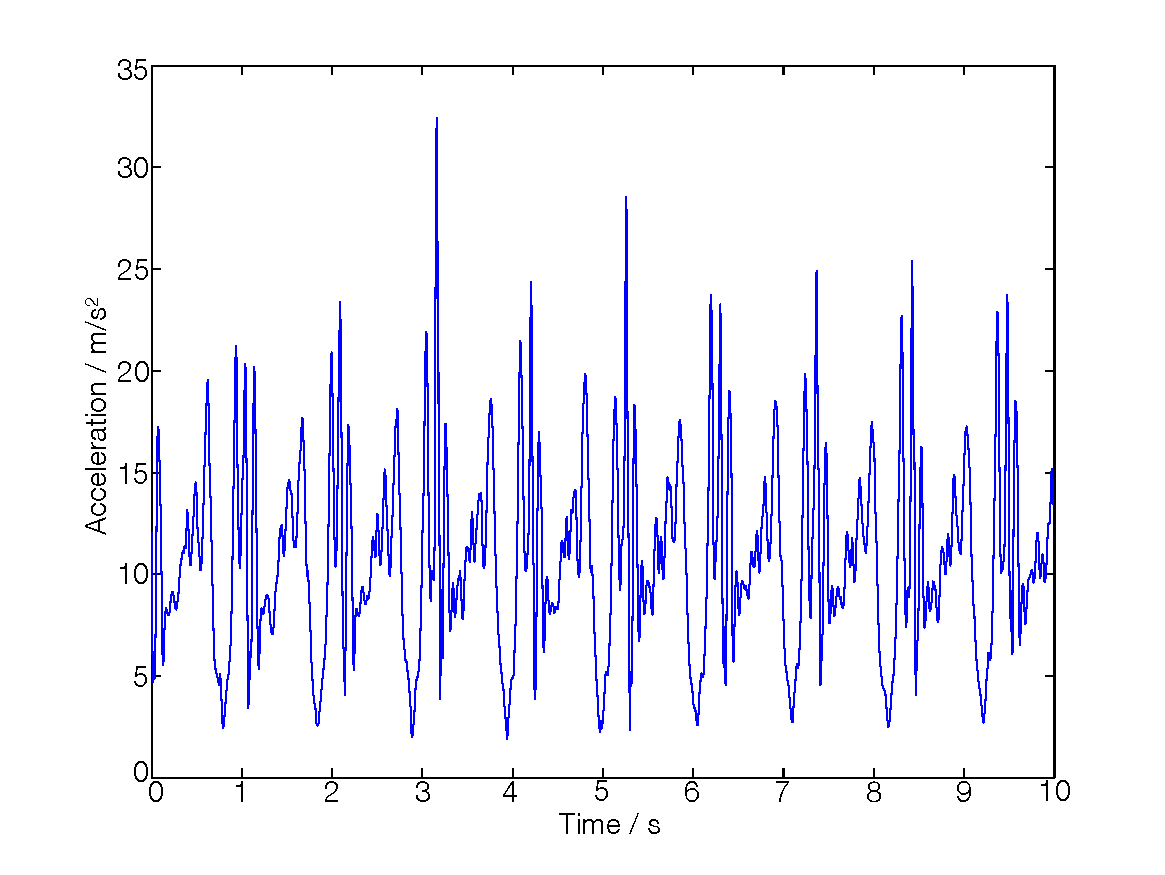
\includegraphics[width=1\textwidth ]{images/kinematic/avr_acc}
\caption{Average acceleration during 10 seconds of a typical walk.}\label{avr_acc}
\end{figure}

A 10 second sample of the average acceleration measured by a phone placed in the front pocket during a typical walk is displayed in figure \ref{avr_acc}. A flaw of this approach is easily noticed, owing to gravity, the average acceleration is centred around this value, ($9.81$ m/s$^2$). A way around this is to differentiate the signal according to 
%
\begin{equation}
\Delta f(x) = \frac{f(x+\Delta t) - f(x) }{\Delta t},
\end{equation} 
%
\begin{figure}[!hbt]
\include{graphics}
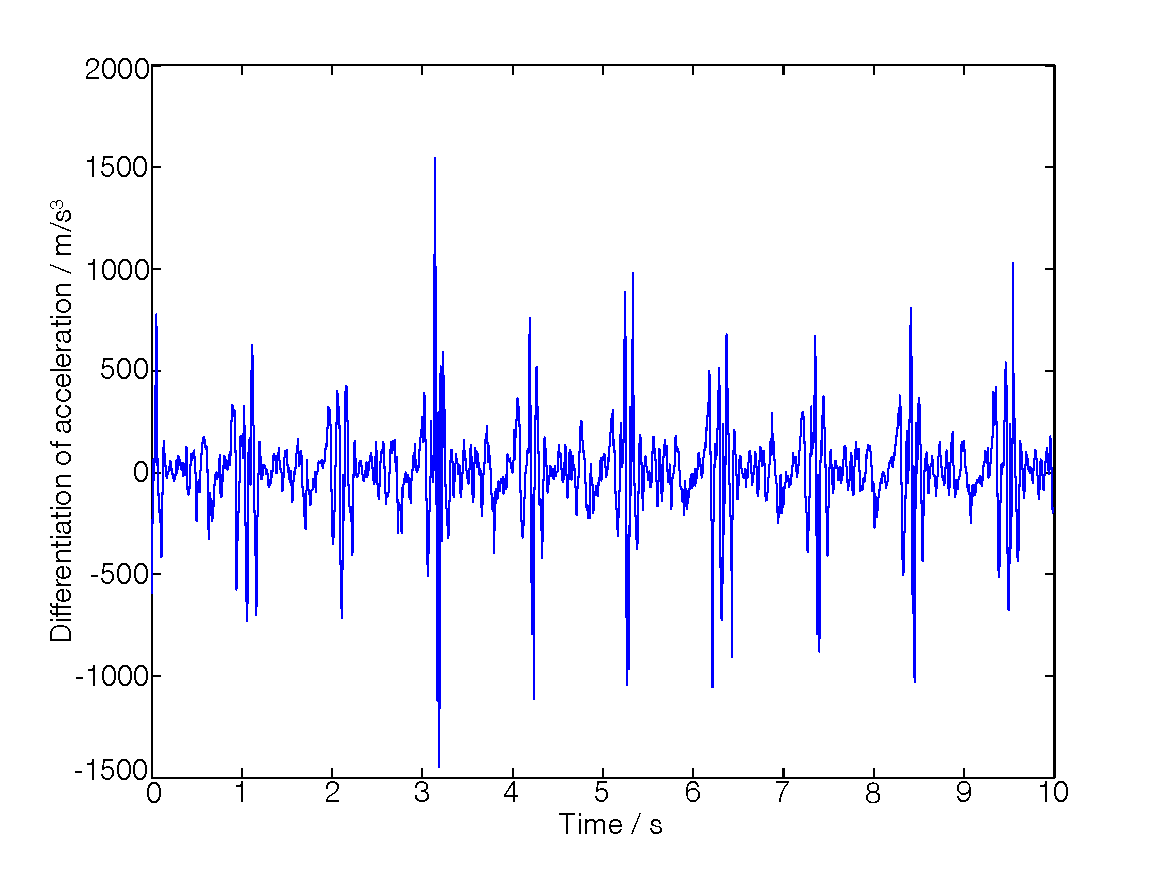
\includegraphics[width=1\textwidth ]{images/kinematic/avr_acc_dif}
\caption{Differentiation of average acceleration during 10 seconds of a typical walk.}\label{avr_acc_dif}
\end{figure}
\subsection{Step Length Considerations}
%
yielding a signal according to figure \ref{avr_acc_dif}. This signal i centred around zero, but possesses unnecessary high frequency behaviour. The sampling frequency for the accelerometer is $\sim 200$ Hz, giving a frequency content of the signal between 0 and 100 Hz. The normal step frequency for a person is no larger than 3 Hz, which promotes filtering the signal. Doing this with a fifth order \emph{Butterworth filter} with a cut-of frequency of 6 Hz yields the signal in figure \ref{avr_acc_dif_filt}.
%
\begin{figure}[!hbt]
\include{graphics}
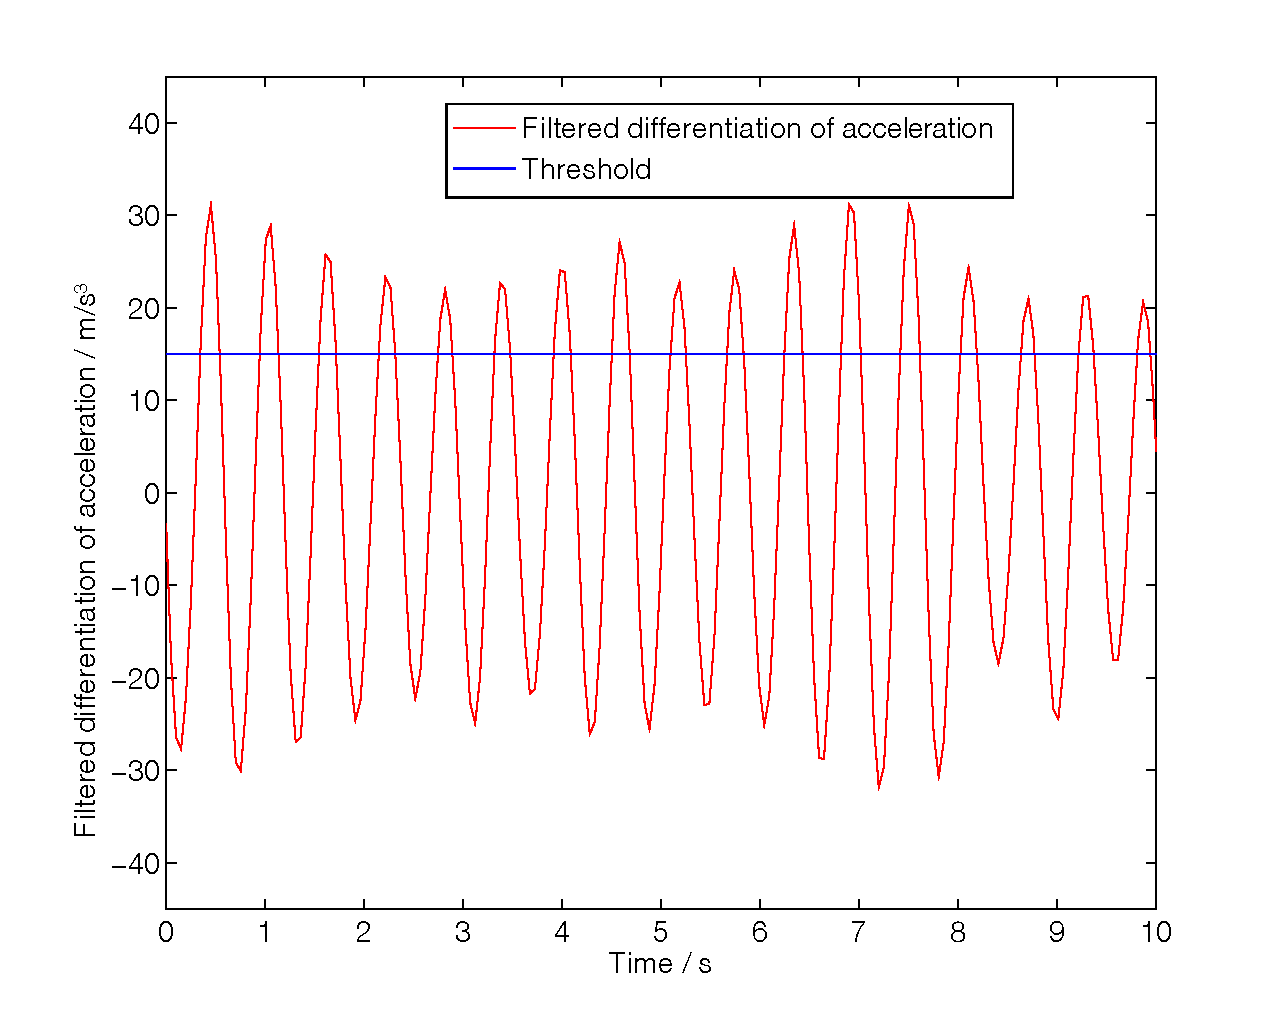
\includegraphics[width=1\textwidth ]{images/kinematic/avr_acc_dif_filt}
\caption{Filtered differentiation of average acceleration during 10 seconds of a typical walk.}\label{avr_acc_dif_filt}
\end{figure}
%
Here the steps are clearly distinguishable, the large peek corresponding to a step with the same leg as the pocket the phone is placed in, the smaller one indicates a step taken by the other leg. A algorithm for identifying a step could be counting the number of times  the signal is decreasing and passing from above to below $-20$.

The technique could be refined further, by e. g identifying the step frequency or by using more sensors. This text more of a short prof of concept for the technique. During the latter parts of this thesis a proprietary solution developed by \emph{Qualcomm} will be used. 
%
\subsection{Step Length Considerations}
%
The step length of an individual, moving in a straight line with a constant speed, is more or less constant. Different individuals or the same individual moving at different speeds or performing turns have a quite large span of step lengths. In this thesis the step length have been determined by the authors walking a predetermined distance comprised of walking straight interspersed with turning both left and right, at a constant speed. The average step length is then simply computed as the distance divided by number of steps and a value of $0.77$ meters was obtained.  

For real world usage however, the length of a users steps must be determined. This can be done in various ways, one is to have the user estimate their own step length but the same method as above. Another is to use adaptive tune the step length by using approximately known distances travelled and the number of steps taken whilst travelling. A way of doing this is to use some sort of positioning technique (GPS, WiFi etc.) to estimate the distance while the step counter determines the number of steps.      
%
\section{Direction of Movement}
%
To have a good estimation of the movement, not only the distance travelled needs to be known. More importantly is the direction in which the movement takes place. In addition, this task is more complicated than finding the distance by the number of steps taken. Many approaches are available using a wide span of technologies, here a some of the mostly used for hand-held devices are presented.  
%
\subsection{Gyroscope}
%
The gyroscope measures the \emph{angular velocities} at which the phone is turning around each of its axis and outputs the values on the format $\vec\omega = (\omega_x \hspace{5pt} \omega_y \hspace{5pt} \omega_z)$. To compute the change of angle, two sets of angular velocities measured with a time difference of $\Delta t$, may be numerically integrated according to the \emph{trapezoidal rule}, 
\begin{equation}
\Delta t \frac{\vec \omega _t +\vec \omega _{t+\Delta t}}{2}.
\end{equation} 
%
There are a few problems of using the gyroscope to determine the direction of movement. As it only measures how the angles change during time, the direction at the start of the navigation must be known and the orientation needs to be kept fixed in reference to the movement. Furthermore, the gyroscope suffers from drifts and biases, so if it is to be used for long stretches of time the heading needs to be calibrated. 
%
\subsection{Magnetometer}
%
A way around the problems of a known initial direction is the use of a magnetometer, which measures the \emph{magnetic field strength} in each of the phones three coordinate directions. Using the known electromagnetic field produced by the earth’s core, it is possible to find the phones heading. In theory this enables the magnetometer along with a known phone orientation to estimate the direction of movement. This is possible in environments where the electromagnetic fields, apart from the earth’s own, is weak, e. g outdoors. In most indoor environments however, fields from electronic devices and structural elements (metal beams, pipes etc.) produced their own magnetic fields. These fields is in many cases strong enough to interfere or even overpower the earth’s, causing the estimated heading to be off. 

The \emph{fingerprinting} strategy for signal strengths described in \ref{sec:AfPA}, may also be utilized to characterize the magnetic field strengths in an indoor environment. These measurements can then be used to find the true heading, but this approach lacks generality as measurements at each location is needed.  
%
\subsection{Sensor Fused Approaches}
%
Different approaches for combining magnetometer, gyroscope and possibly other sensors to produce a sensor fused estimation of the heading. Most Android phones implements such an algorithm, using gyroscope, magnetometer and accelerometer to produce an estimate of how the phone is oriented in the world coordinate system. The algorithm uses gyroscope and accelerometer to determine when the magnetometer output is corrupted, and uses their measurements to estimate the heading until the magnetometer can be trusted. ASK ABOUT HOW THIS WORKS IN PRACTICE!!!
%
\section{Dead Reckoning}
%
\emph{Dead reckoning} is the process of calculating the current position based on a previously determined position and advancing that position based on a known model. Dead reckoning has been used by e. g ships and airplanes for a long time or in more resent time in networked computer games. 

Dead reckoning estimations are subject to cumulative errors i. e errors are added over time and depending on the accuracy of the dead reckoning system, the estimated position deviates from the true. This imply that the position estimate and heading needs to be calibrated at a certain time interval to provide an  accurate position.

For phones a dead reckoning estimation would most likely include some form of step counting combined with one of the heading estimations previously mentioned. As an example, the true and estimated path using a pedometer and a gyroscope during a walk of approximately 110 meters, is presented in figure \ref{deadreckon_1}. The behaviour is fairly good but there is a heading error present soon after the start, and this grows as the walk continues. The distance estimated by the pedometer is also larger than the true distance travelled.  
%
\begin{figure}[!hbt]
\include{graphics}
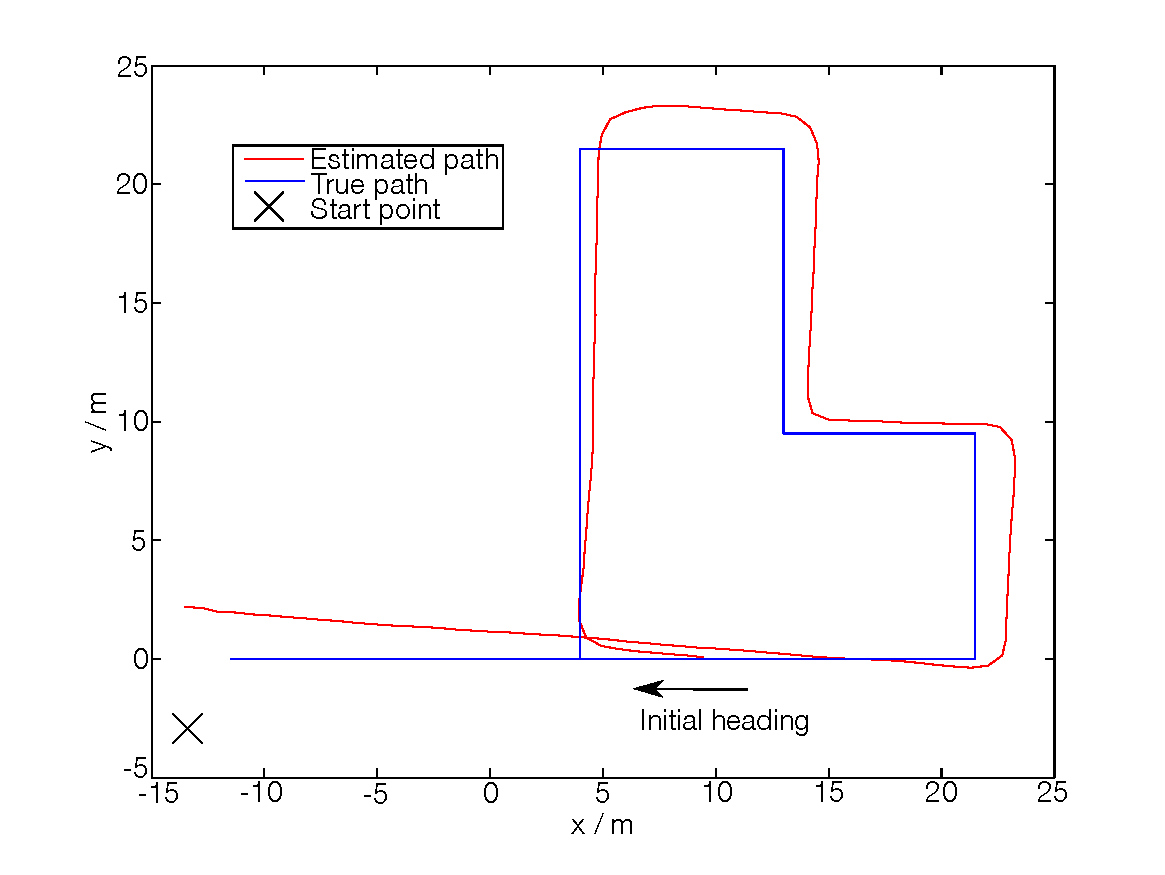
\includegraphics[width=1\textwidth ]{images/kinematic/deadreckon_1}
\caption{True versus, by dead reckoning, estimated path using gyroscope and pedometer.}\label{deadreckon_1}
\end{figure}

However, as stated before, the error in cumulative and the performance deteriorates with time. This is shown in figure \ref{deadreckon_2}. The distance round the rectangle is approximately 105 meters and the especially the heading error is clearly visible. 
%
\begin{figure}[!hbt]
\include{graphics}
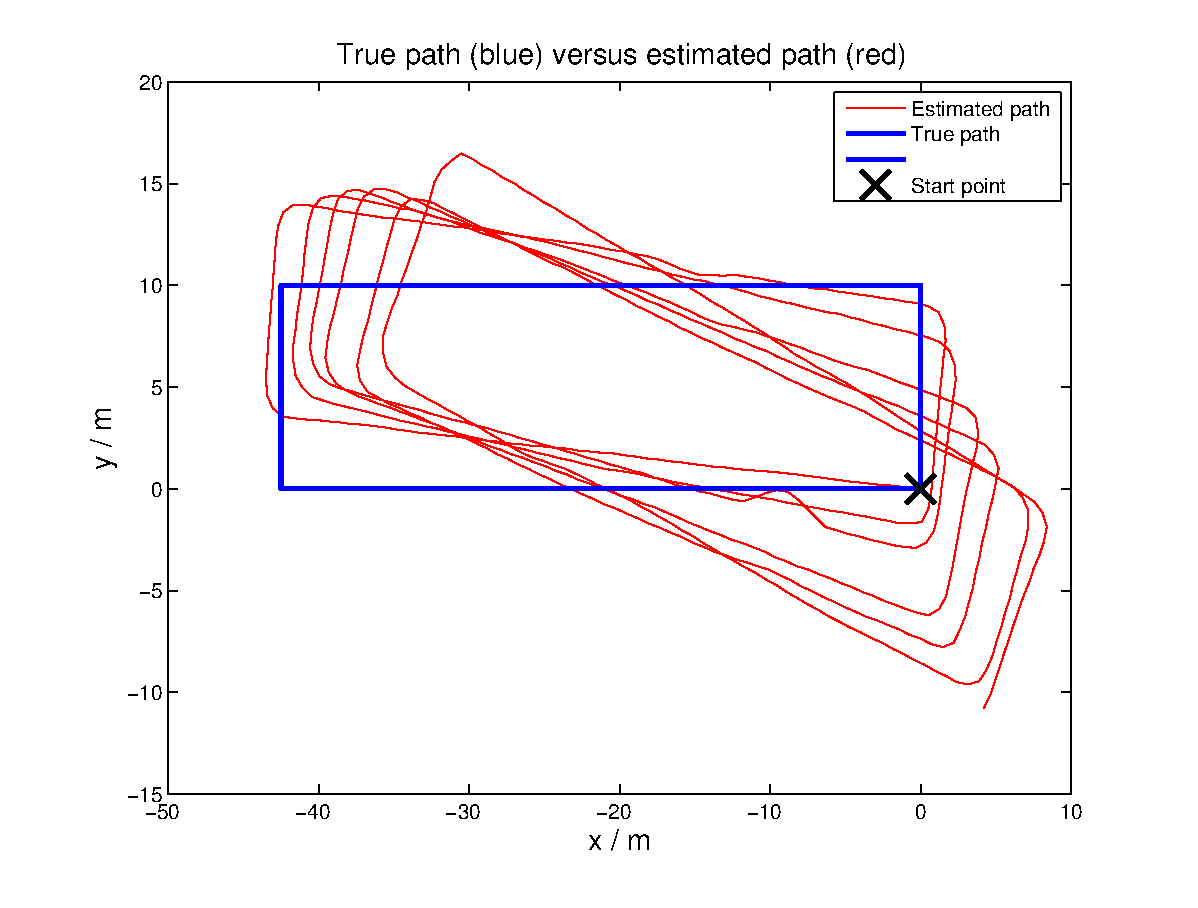
\includegraphics[width=1\textwidth ]{images/kinematic/deadreckon_2}
\caption{True versus, by dead reckoning, estimated path using gyroscope and pedometer.}\label{deadreckon_2}
\end{figure}

SOME ABOUT THE ROTATION VECTORS HERE

It is apparent that both position and heading needs to be calibrated to obtain a good position estimate. How this is done is explained in the following chapters.
%
\chapter{Sensor Evaluation}
%
\chapter{Indoor positioning - Sensor Fused Approach} 

\printbibliography  %% Comment if you don't want to use bibtex

\end{document}





